% -*- coding: utf-8 -*-
% !TEX encoding = UTF-8 Unicode
% !TEX root =  main.tex

\chapter{Auswertung der Simulation}
\label{chap:ergebnisse-foc}

In diesem Kapitel sollen die Ergebnisse der durchgeführten Simulation aus den Kapitel~\ref{cha:regelungpmsm} diskutiert werden.
%Dabei werden dem Leser Simulationsergebnisse und Probleme gezeigt, diese konnten aufgrund des Zeitaufwandes nicht mehr gelöst werden.
Zu den ausgewählten Lösungsverfahren (s.~h.~Abschnitt~\ref{sec:parameter}) wurde das Runge-Kutta-Verfahren mit fester Schrittweite gewählt.

\section{Model and simulation parameter}\label{sec:parameter}

Wie schon in der Einleitung dargestellt, wurde das Runge-Kutta\footnote{Nach Carl Runge und Martin Wilhelm Kutta benannt.}-Verfahren gewählt.
Dieses Verfahren ist ein sog. Einzelschrittverfahren zur näherungsweisen Lösung von Anfangswertproblemen in der numerischen Mathematik.
Gegeben sei das Anfangswertproblem

\begin{align}
	y'(t) = f(t,y(t)), y(t_\x{0})=y_\x{0}, y: \mathbb{R}\rightarrow\mathbb{R}^{d}
\end{align}

mit exakter Lösung $y(t)$.
Die exakte Lösung kann im Allgemeinen nicht angegeben werden, weshalb man sich mit einer Näherung, wie Runge-Kutta-Verfahren annährt.
Die $s$-stufigen Runge-Kutta-Verfahren sind Einschrittverfahren, die durch Ausdrücke der folgenden Art gegeben sind

\begin{align}
	y_{n+1} = y_n + h \sum_{j=1}^{s}{b_j k_j}
\end{align}

Dabei bezeichnet $h$ die Schrittweite zwischen den aufeinanderfolgenden Stützstellen $t_n$ und $t_{n+1}$.
Die Koeffizienten $b_j$ definieren das jeweilige Verfahren und können als Quadraturformel für das Integral

\begin{align}
	\int_{t_n}^{t_{n+1}}{f(t,y(t))dt}
\end{align}

interpretiert werden.
Die Größen $k_j$ bezeichnet man als Zwischenschritt, sie entsprechen Auswertungen der rechten Seite von $f$ an bestimmten Stellen.
Die Steuerung der Schrittweite $h$ ist von besonderem Interesse.
Man kann sich leicht vorstellen, dass die Funktion in Bereichen, in denen nur geringe Änderungen zwischen $y_{n+1}$ und $y_n$ vorliegen, mit weniger Rechenschritten auskommt, als in solchen, in den schnelle Änderungen vorliegen.\footnote{Vgl.~W.\ Kutta: \enquote{Beitrag zur näherungsweisen Integration totaler Differenzialgleichungen}, Z. Math. Phys., Bd. 46, 1901, S.~425--453}\footnote{Vgl.~C.\ Runge: \enquote{Über die numerische Auflösung von Differenzialgleichungen}, Math. Annalen, Bd. 46, 1895, S.~167--178, Online \url{http://gdz.sub.uni-goettingen.de/dms/load/img/?PPN=PPN235181684_0046&DMDID=DMDLOG_0022}}


\begin{table}[h!]
	\centering
	\caption{Model configuration parameters.}
	\label{tab:model-parameter}
	\begin{tabularx}{0.8\textwidth}{ll}
		\toprule
		Beschreibung: & Eingestellter Wert: \\
		\midrule
		Solver options	& Fixed Step\\
		Fixed-step size (fundamental sample time)	& 1e-6 \\
		Solver	& ode4 (Runge-Kutta) \\
		Start time & 0.0 \\
		Stop time & 10.0\\
		Periodic sample time constraint & Unconstrained \\
		Tasking mode for periodic sample times & Auto \\
		\bottomrule
	\end{tabularx}
\end{table}
\begin{table}[h!]
	\centering
	\caption{PMSM model configuration parameter.}
	\label{tab:pmsm-parameter}
	\begin{tabularx}{0.8\textwidth}{ll}
		\toprule
		Beschreibung: & Eingestellter Wert: \\
		\midrule
		Trägheitsmoment $J$ & \SI{0.062}{\kilogram\square\meter} \\
		Frequenz $f$ & \SI{50}{\hertz}\\
		Induktivität in $d,q$-Richtung ($L_\x{d}=L_\x{q}$) & \SI{0.0085}{\ohm\second}\\
		Polpaarzahl $p$ & 4 \\
		Flussverkettung $\Psi_\x{pm}$ & \SI{0.0715}{\volt\second}\\
		Ständerwiderstand $R_\x{1}$ & \SI{0.18}{\ohm}\\
		Drehzahl Sollwert $n_\x{soll}$ & \SI{500}{\per\minute}\\
		Drehmoment Sollwert $M_\x{Last}$ & \SI{60}{\newton\meter}\\
		\bottomrule
	\end{tabularx}
\end{table}
%\verylongpage
\newpage

\section{Simulationsergebnisse ohne Netz}\label{sec:sim-ohne-netz}

In diesem Abschnitt werden die Ergebnisse der Simulation ohne Netz dargestellt.

\begin{figure}[h!]
\begin{minipage}[t]{0.5\textwidth}
		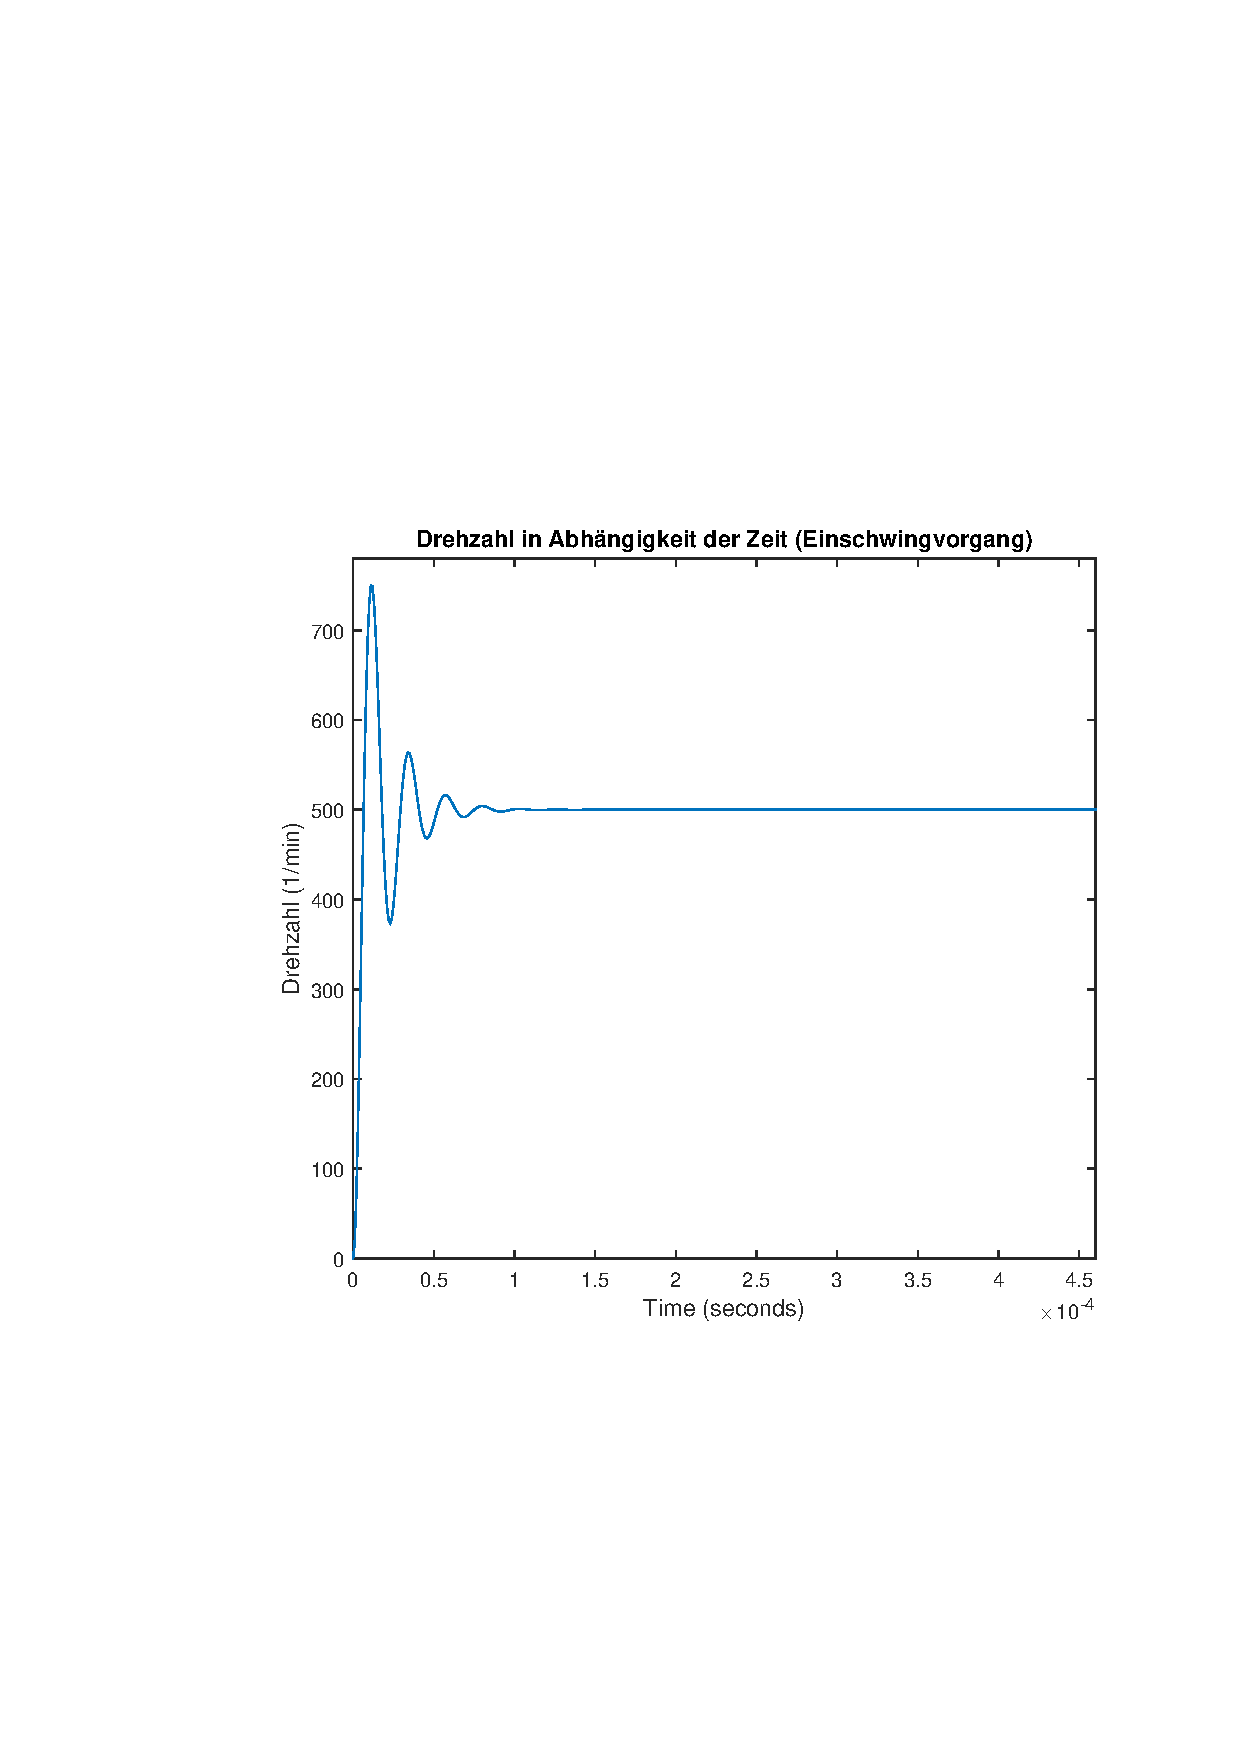
\includegraphics[width=\textwidth]{erg/drehzahl-einschwingvorgang.pdf}
\end{minipage}
\begin{minipage}[t]{0.5\textwidth}
		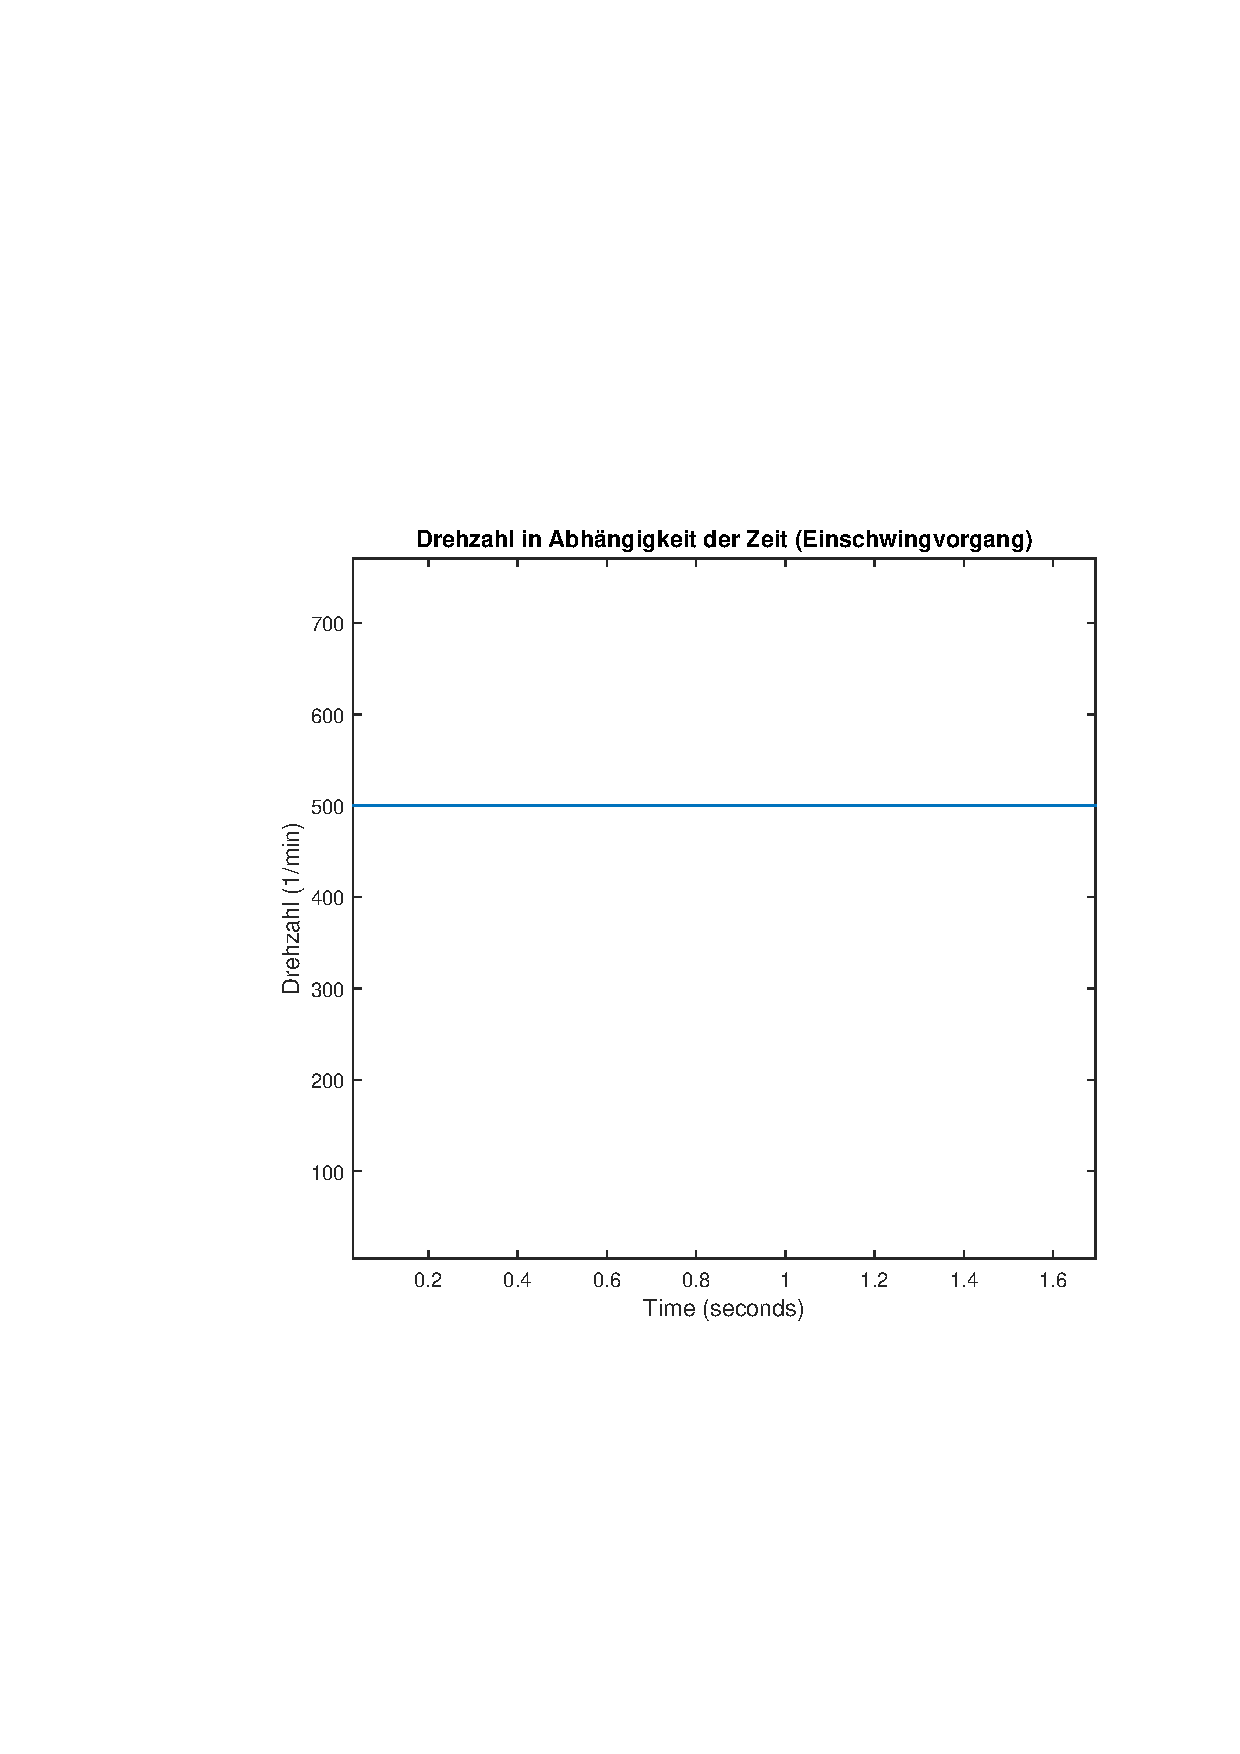
\includegraphics[width=\textwidth]{erg/drehzahl-einschwingvorgang-2.pdf}
\end{minipage}
\caption{Drehzahl in Abhängigkeit der Zeit, Einschwingvorgang.}
\label{fig:drehzahl-einschwingvorgang}
\end{figure}

Wie in Abbildung \ref{fig:drehzahl-einschwingvorgang} erkennbar, regelt das System die Drehzahl auf \SI{500}{\per\minute}.

\begin{figure}[h!]
\begin{minipage}[t]{0.5\textwidth}
	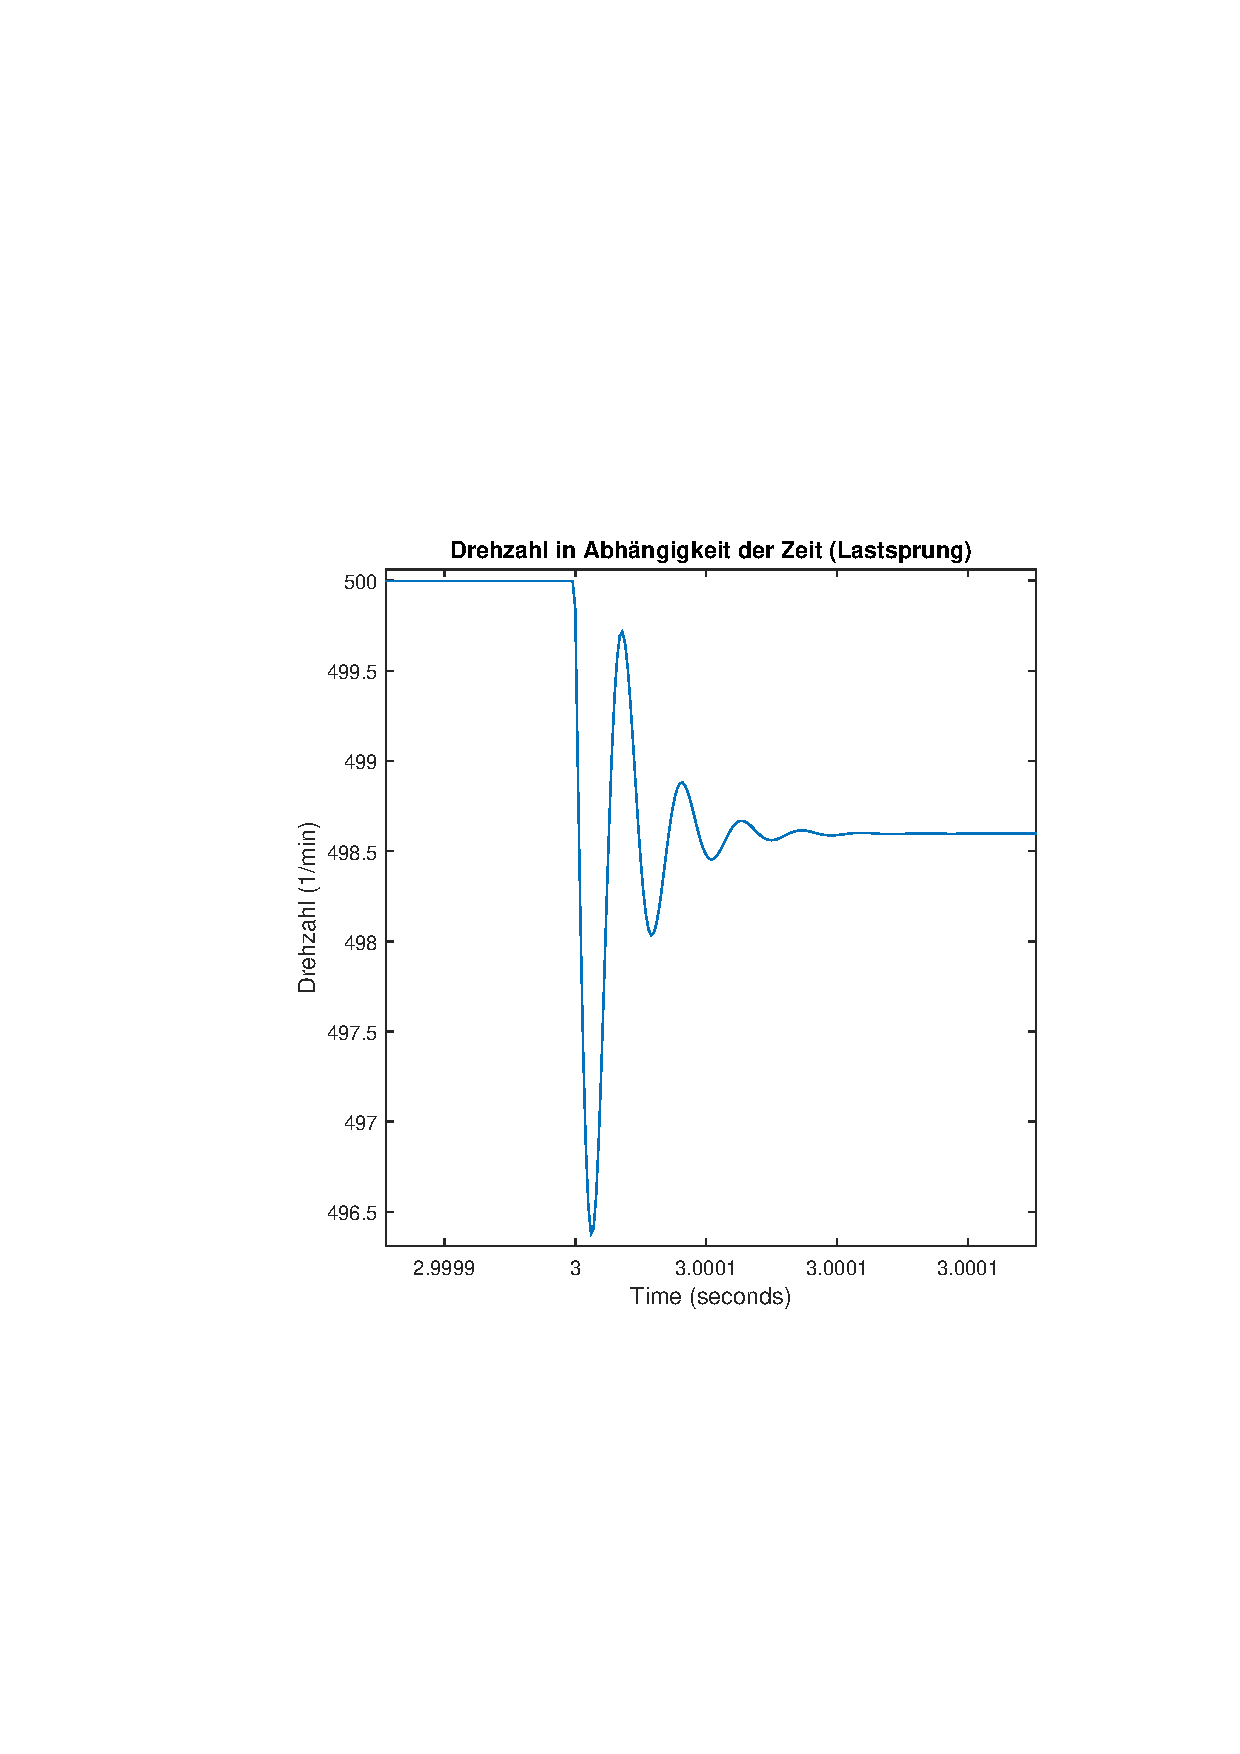
\includegraphics[width=\textwidth]{erg/drehzahl-lastsprung-1.pdf}
\end{minipage}
\begin{minipage}[t]{0.5\textwidth}
	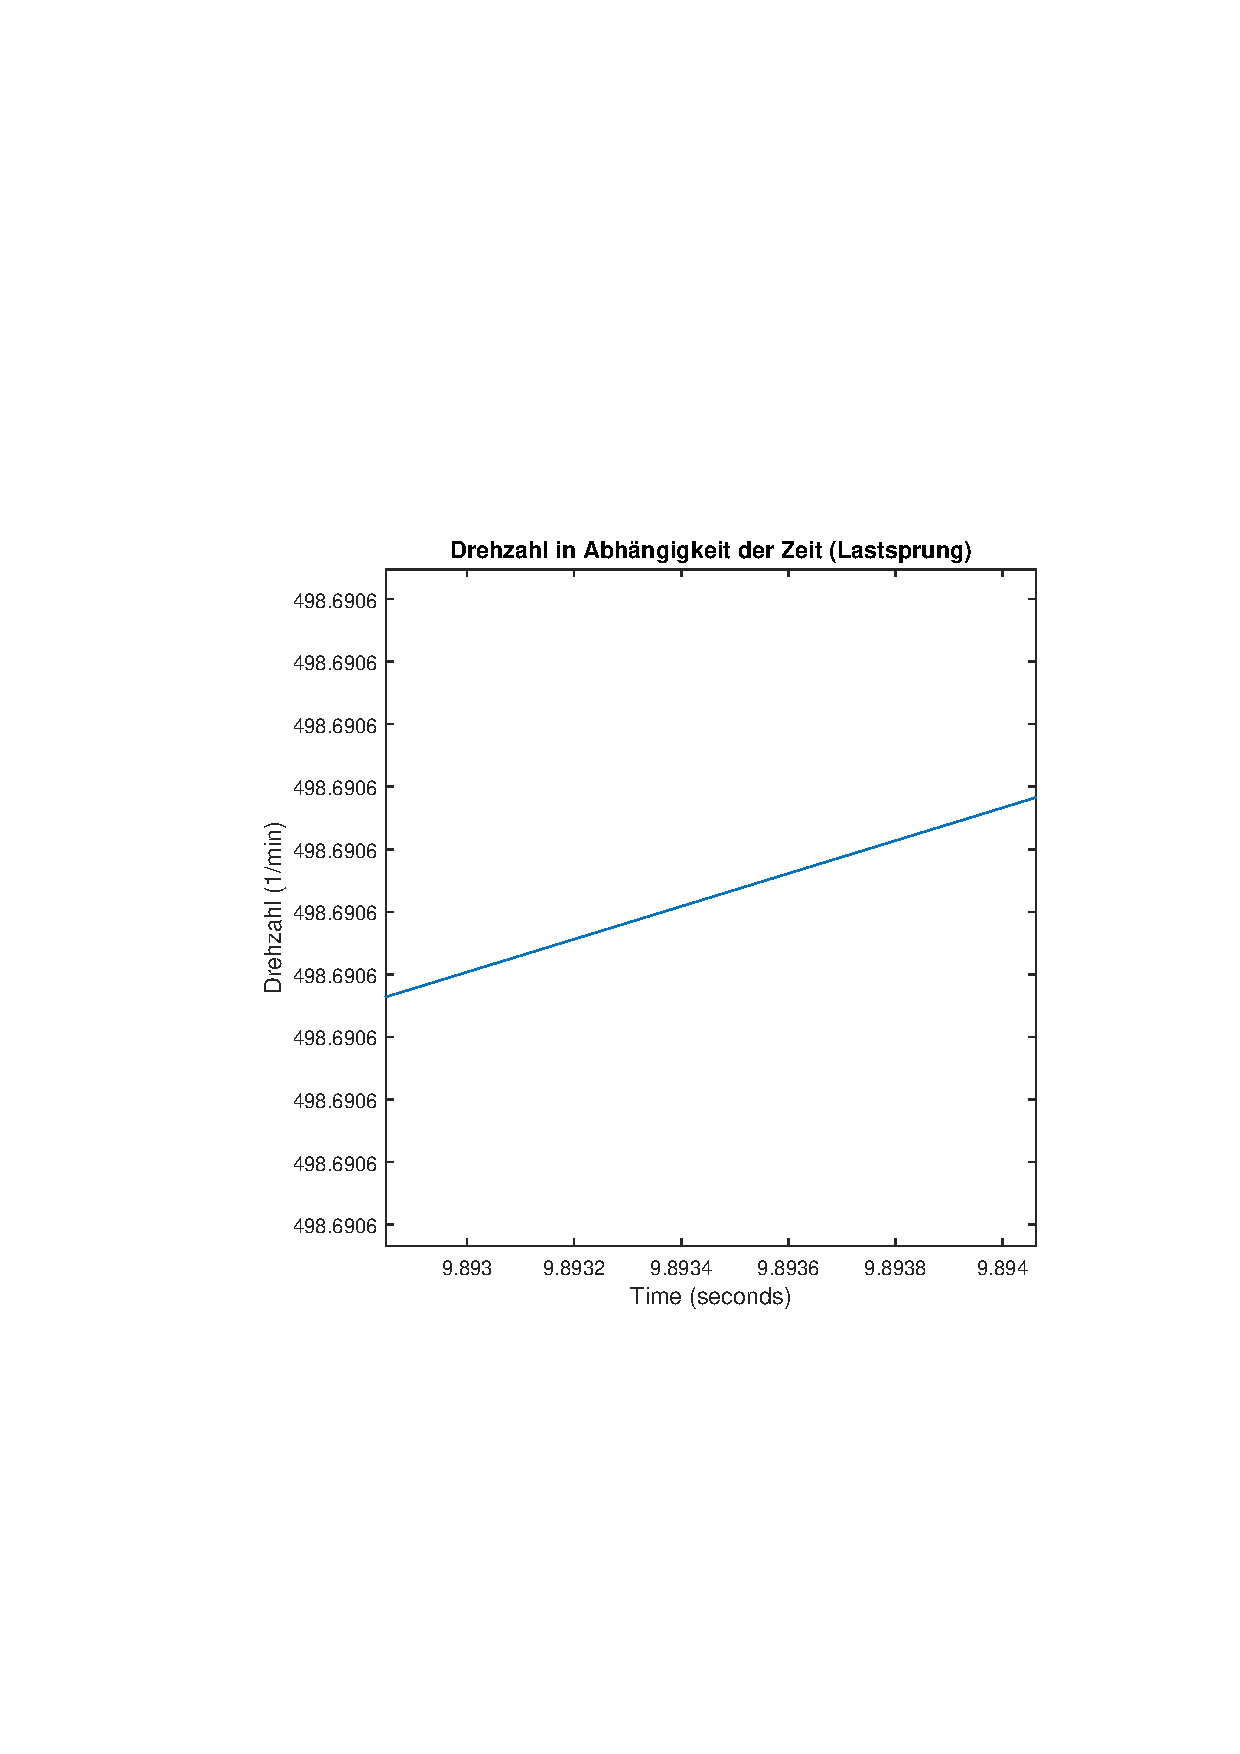
\includegraphics[width=\textwidth]{erg/drehzahl-lastsprung-2.pdf}
\end{minipage}
\caption{Drehzahl in Abhängigkeit der Zeit, Ausschnitt: Lastsprung.}
\label{fig:drehzahl-lastsprung}
\end{figure}
 
Nach Zugabe des Lastsprunges (nach \SI{3}s mit einem Drehmomentsollwert von \SI{60}Nm) regelt das System die Drehzahl auf \SI{498.5}{\per\minute}.
Der flussverursachende Strom $(i_\x{d})$ der Maschine ändert sich durch die Drehmomentvorgabe so, dass dieser länger braucht um auf null geregelt zu werden.
 
%In Abbildung \ref{fig:drehzahl-lastsprung} ist erkennbar, dass sich die Maschine sich nach längerer Simulationszeit erst kurz vor den \SI{500}{\per\minute} einpendelt, dies liegt zum einen an den eingestellten Regelparametern der Simulation und zum anderen weil sich der Fluss der Maschine nur sehr langsam ändern kann.

\begin{figure}[h!]
	\begin{minipage}[t]{0.5\textwidth}
		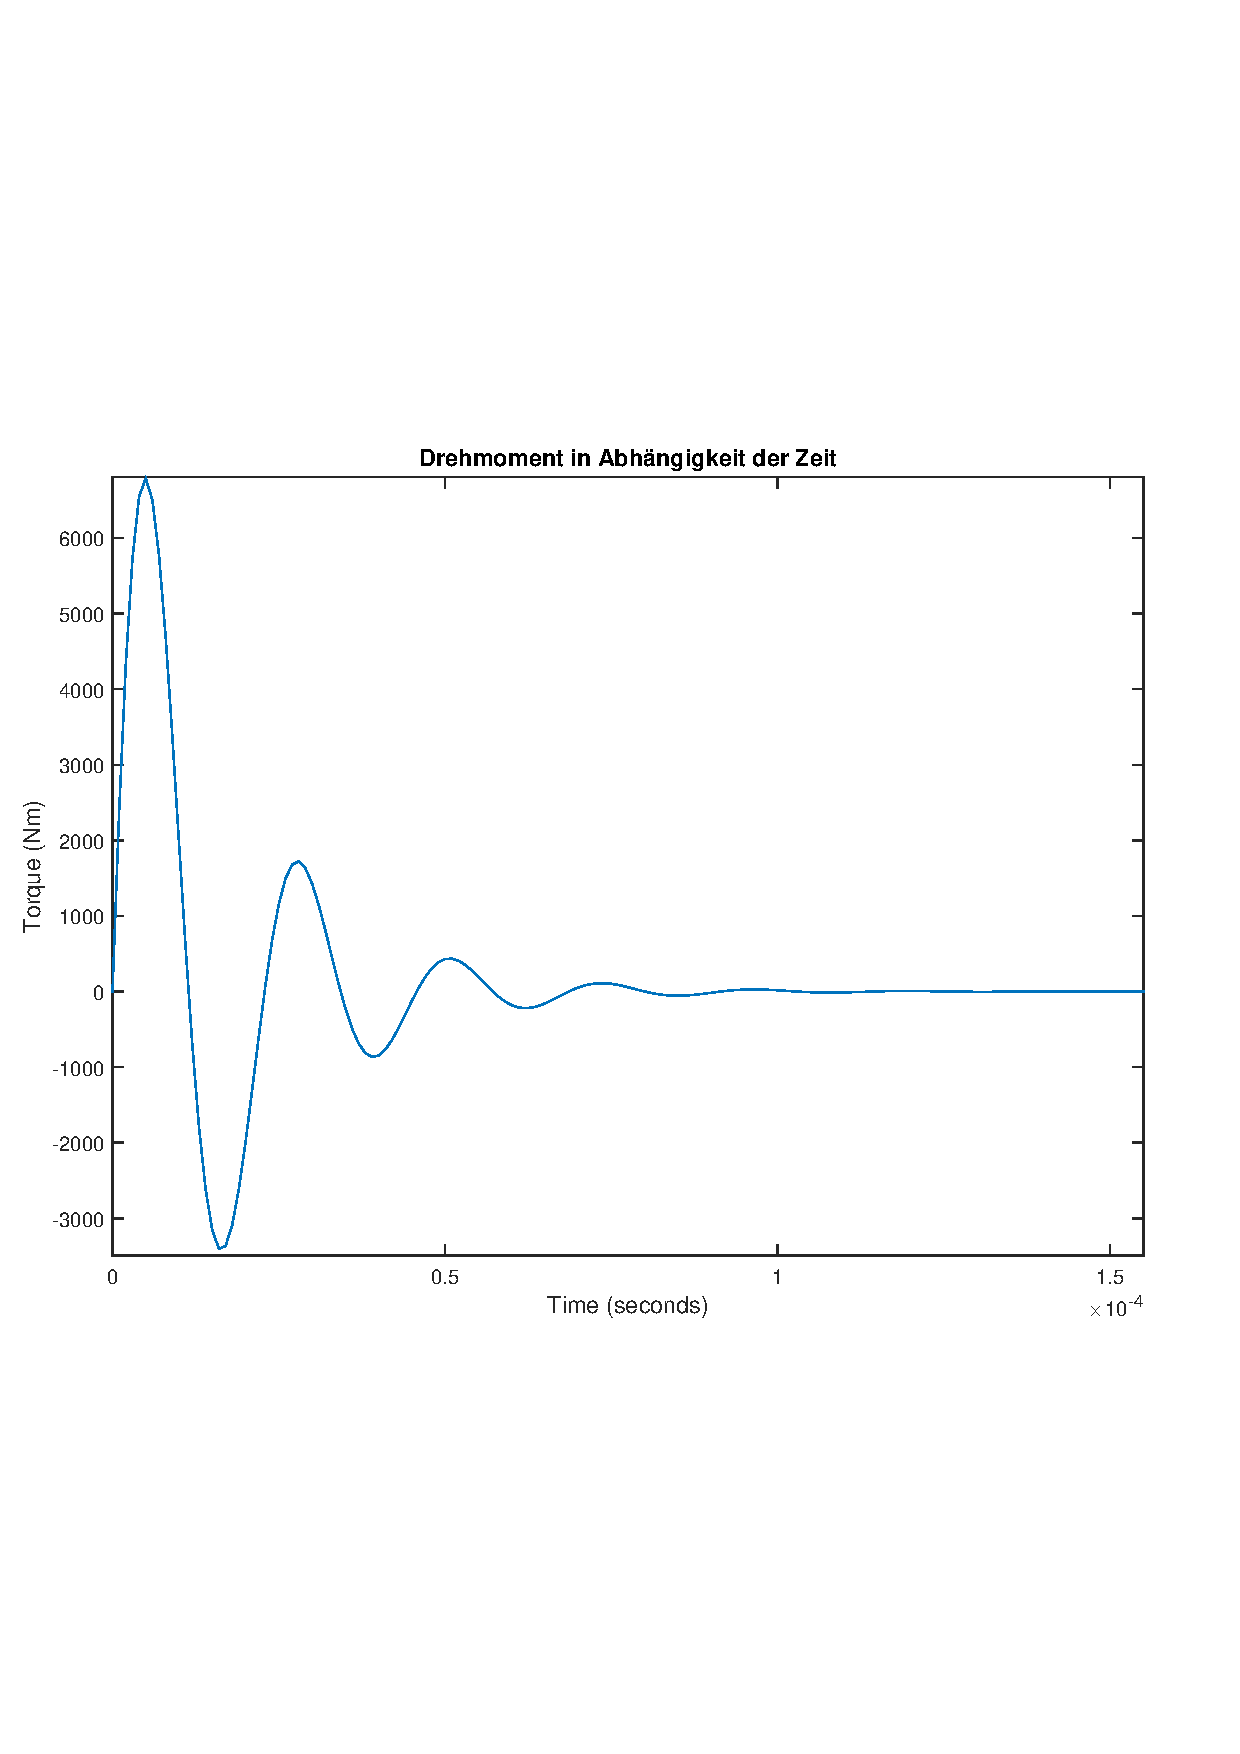
\includegraphics[width=\textwidth]{erg/drehmoment-einschwing.pdf}
	\end{minipage}
	\begin{minipage}[t]{0.5\textwidth}
		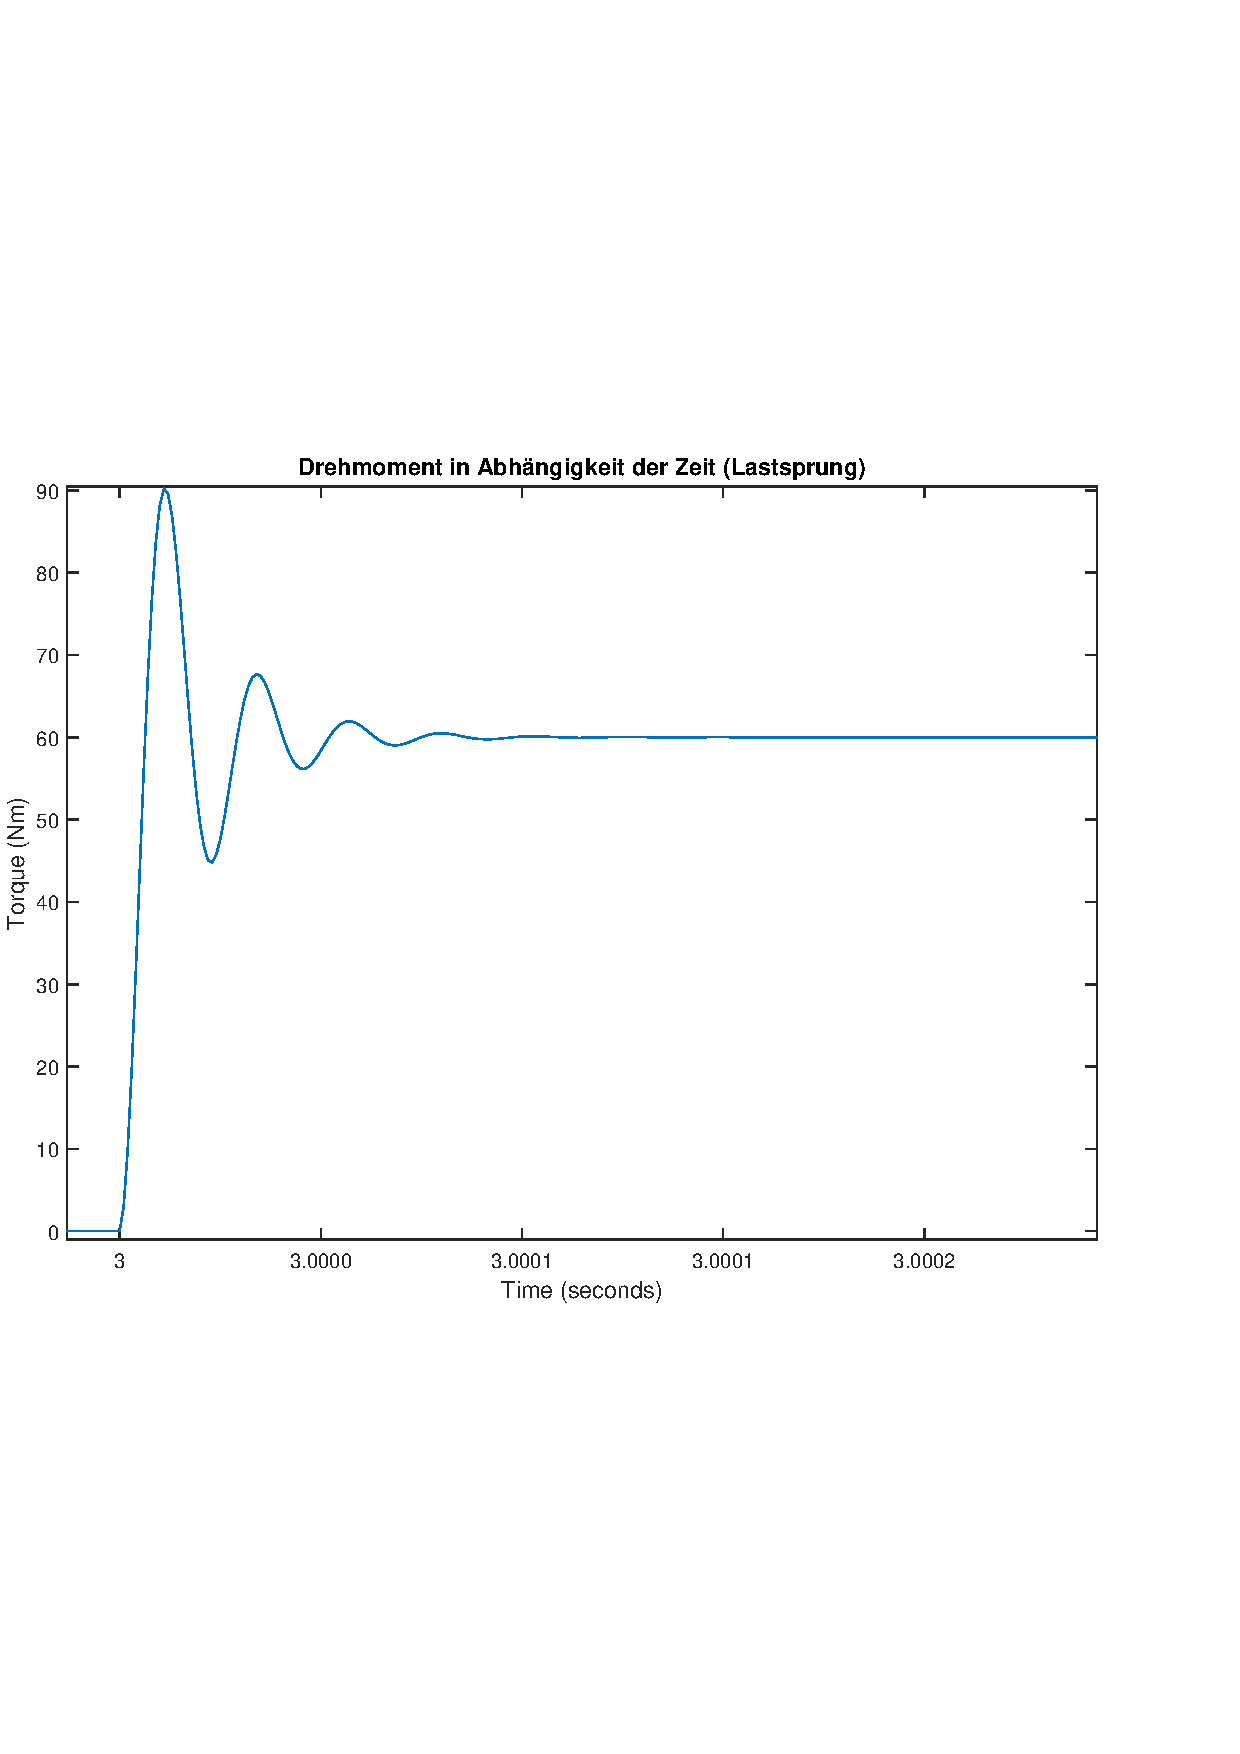
\includegraphics[width=\textwidth]{erg/drehmoment-lastsprung.pdf}
	\end{minipage}
	\caption{Drehmoment in Abhängigkeit der Zeit. Links: Einschwingvorgang. Rechts: Lastsprung.}
	\label{fig:drehmoment}
\end{figure}

In kürzester Zeit schwingt sich das System ein (s.~h.~Abbildung~\ref{fig:drehmoment}).
Den Lastsprung regelt das System in kürzester Zeit aus, sodass sich das Drehmoment von \SI{60}Nm einstellt.

\begin{figure}[h!]
	\begin{minipage}[t]{0.5\textwidth}
		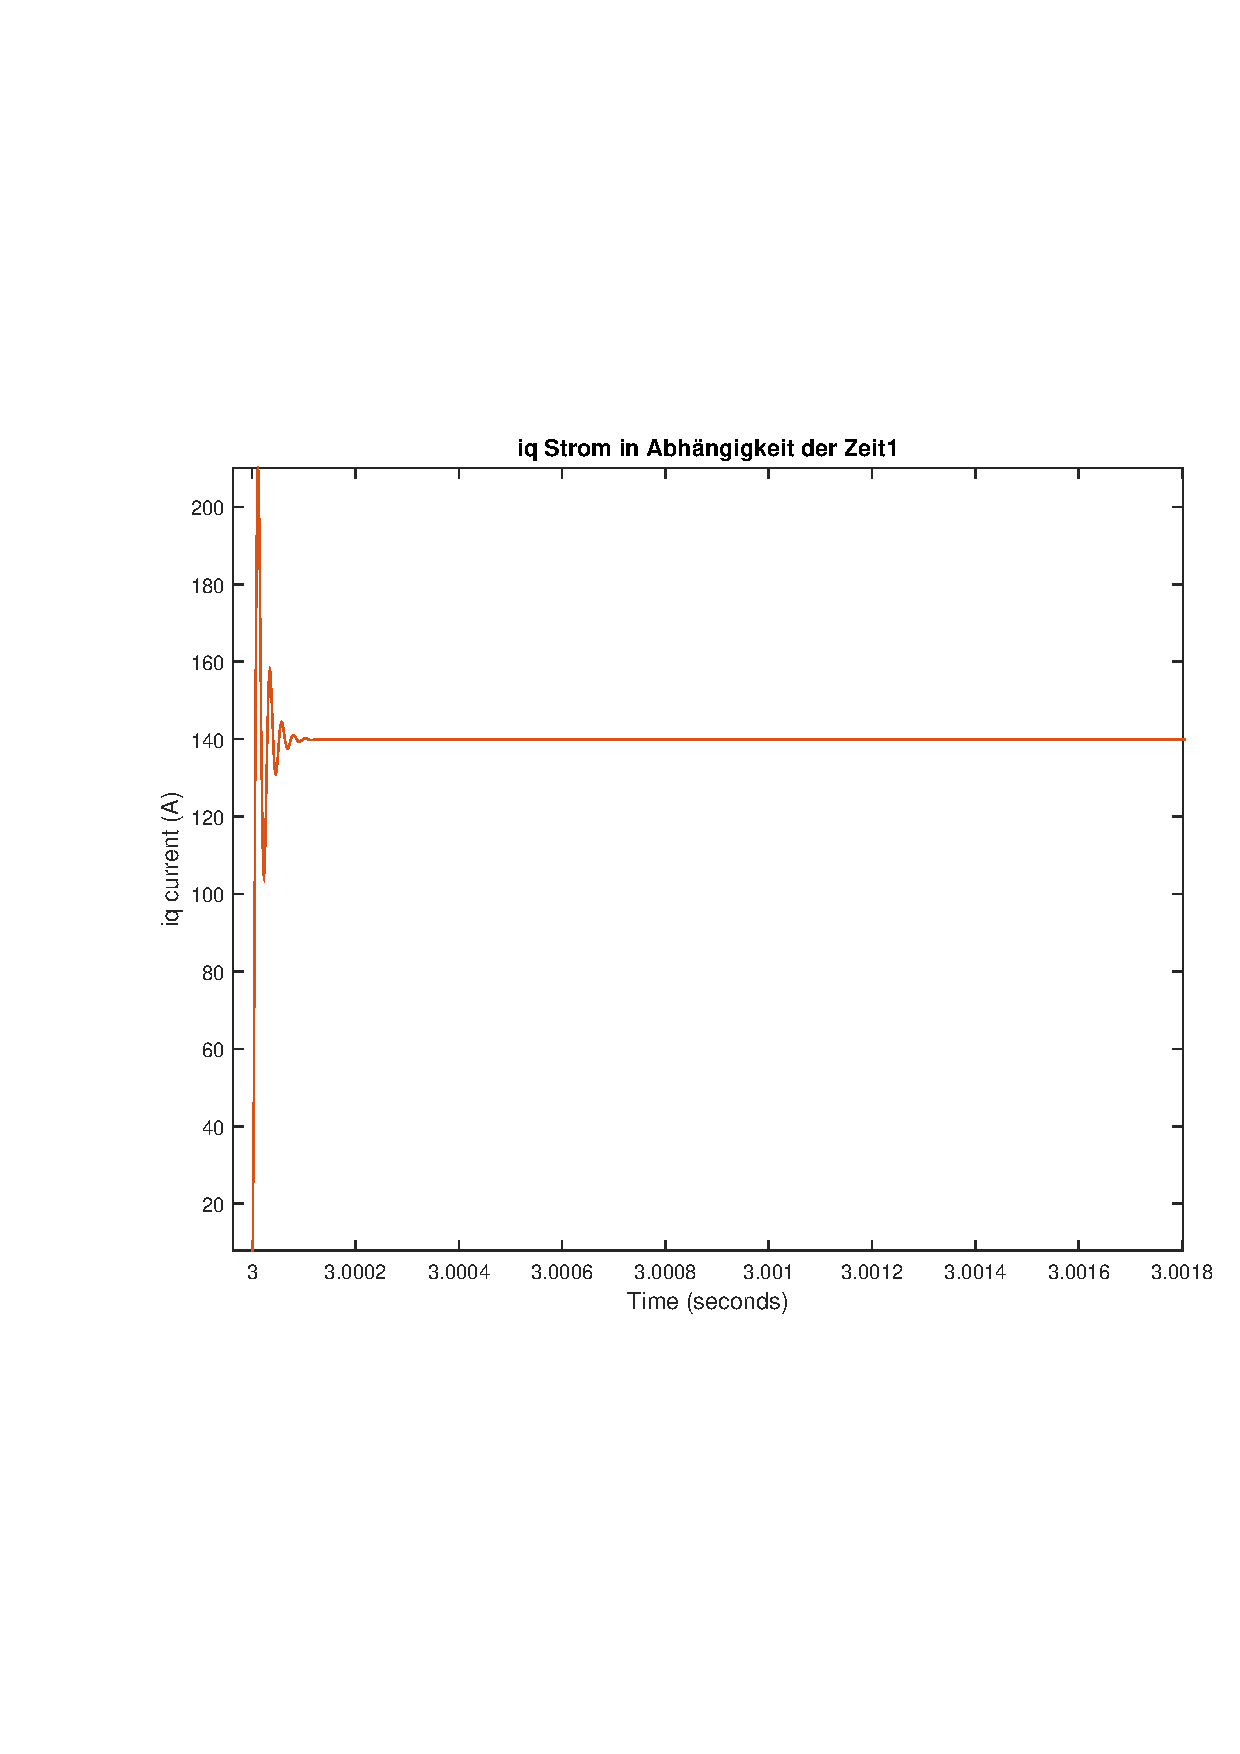
\includegraphics[width=\textwidth]{erg/iq.pdf}
	\end{minipage}
	\begin{minipage}[t]{0.5\textwidth} 
		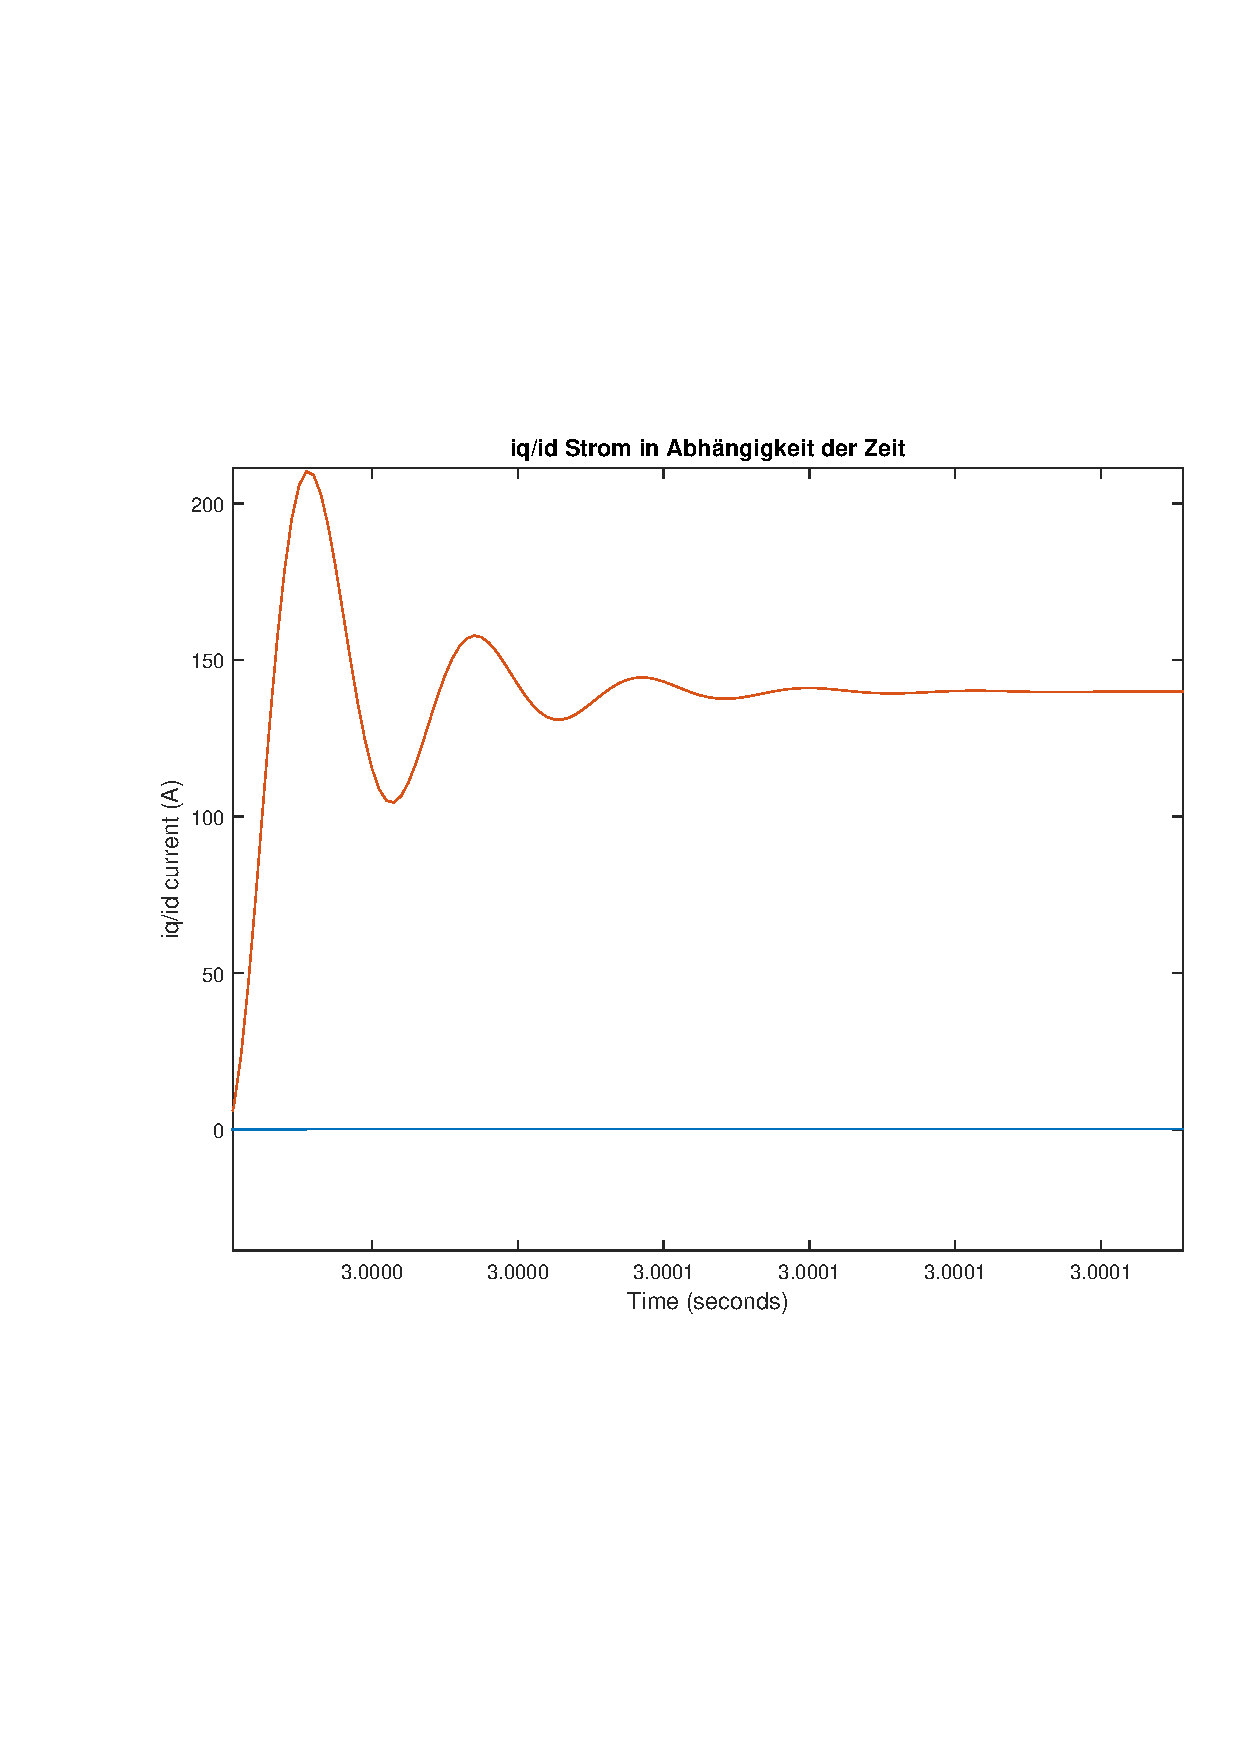
\includegraphics[width=\textwidth]{erg/idiq.pdf}
	\end{minipage}
		\caption{Ströme der Maschine graphisch dargestellt.}
		\label{fig:idiq-strom}
	\end{figure}

Wie schon beim Drehmoment (s.~h.~Abbildung~\ref{fig:drehmoment}) erkennbar, regelt das System den $i_\x{q}$-Strom so, dass das Drehmoment auf \SI{60}Nm geregelt wird (s.~h.~Abbildung~\ref{fig:idiq-strom}).
In Abbildung \ref{fig:idiq-strom} rechts, ist der $i_\x{d}$- und $i_\x{q}$-Strom aufgetragen.
Der $i_\x{d}$-Strom wird vom System auf Null geregelt.

\newpage

\section{Simulationsergebnisse am starren Netz}\label{sec:sim-starr-netz}

\begin{figure}[h!]
	\begin{minipage}[t]{0.5\textwidth}
		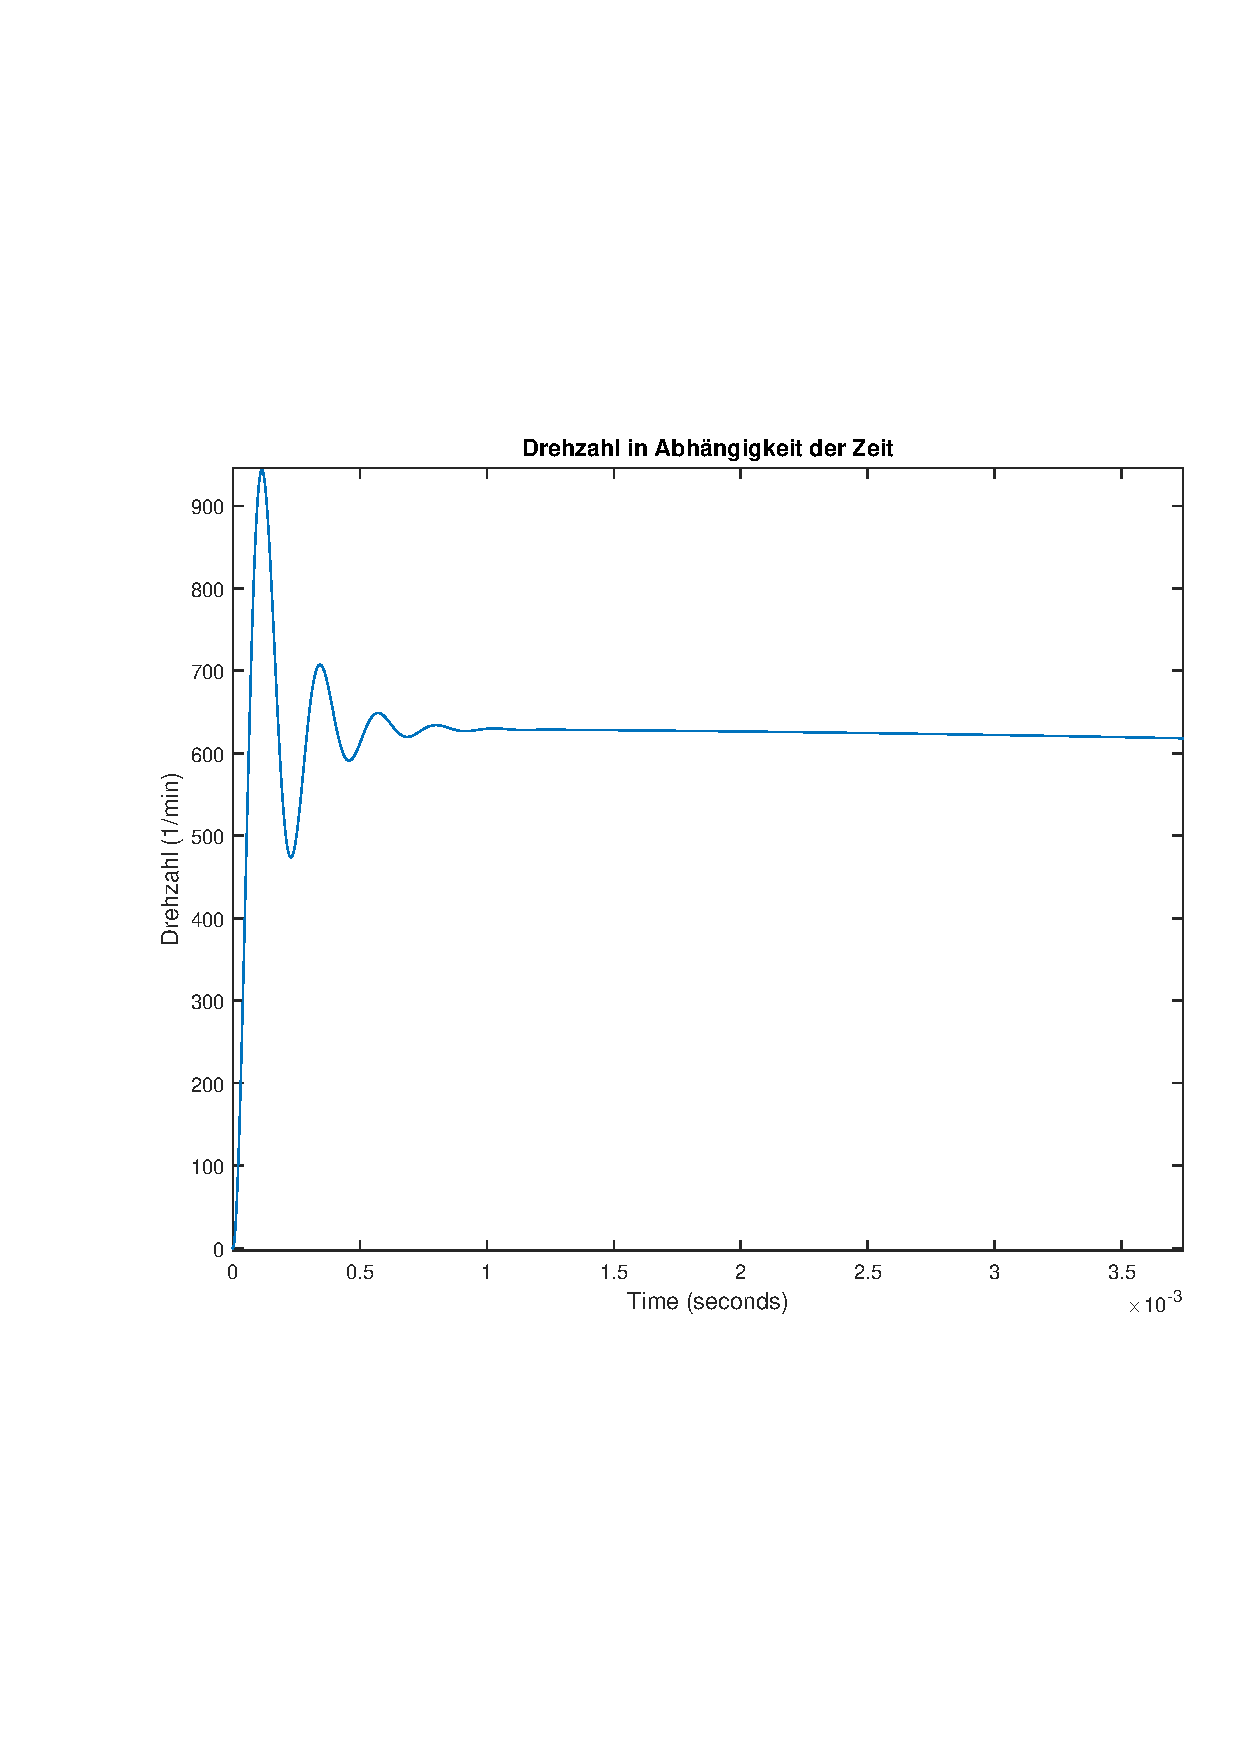
\includegraphics[width=\textwidth]{erg/netz/drehzahl-netz-1.pdf}
	\end{minipage}
	\begin{minipage}[t]{0.5\textwidth} 
		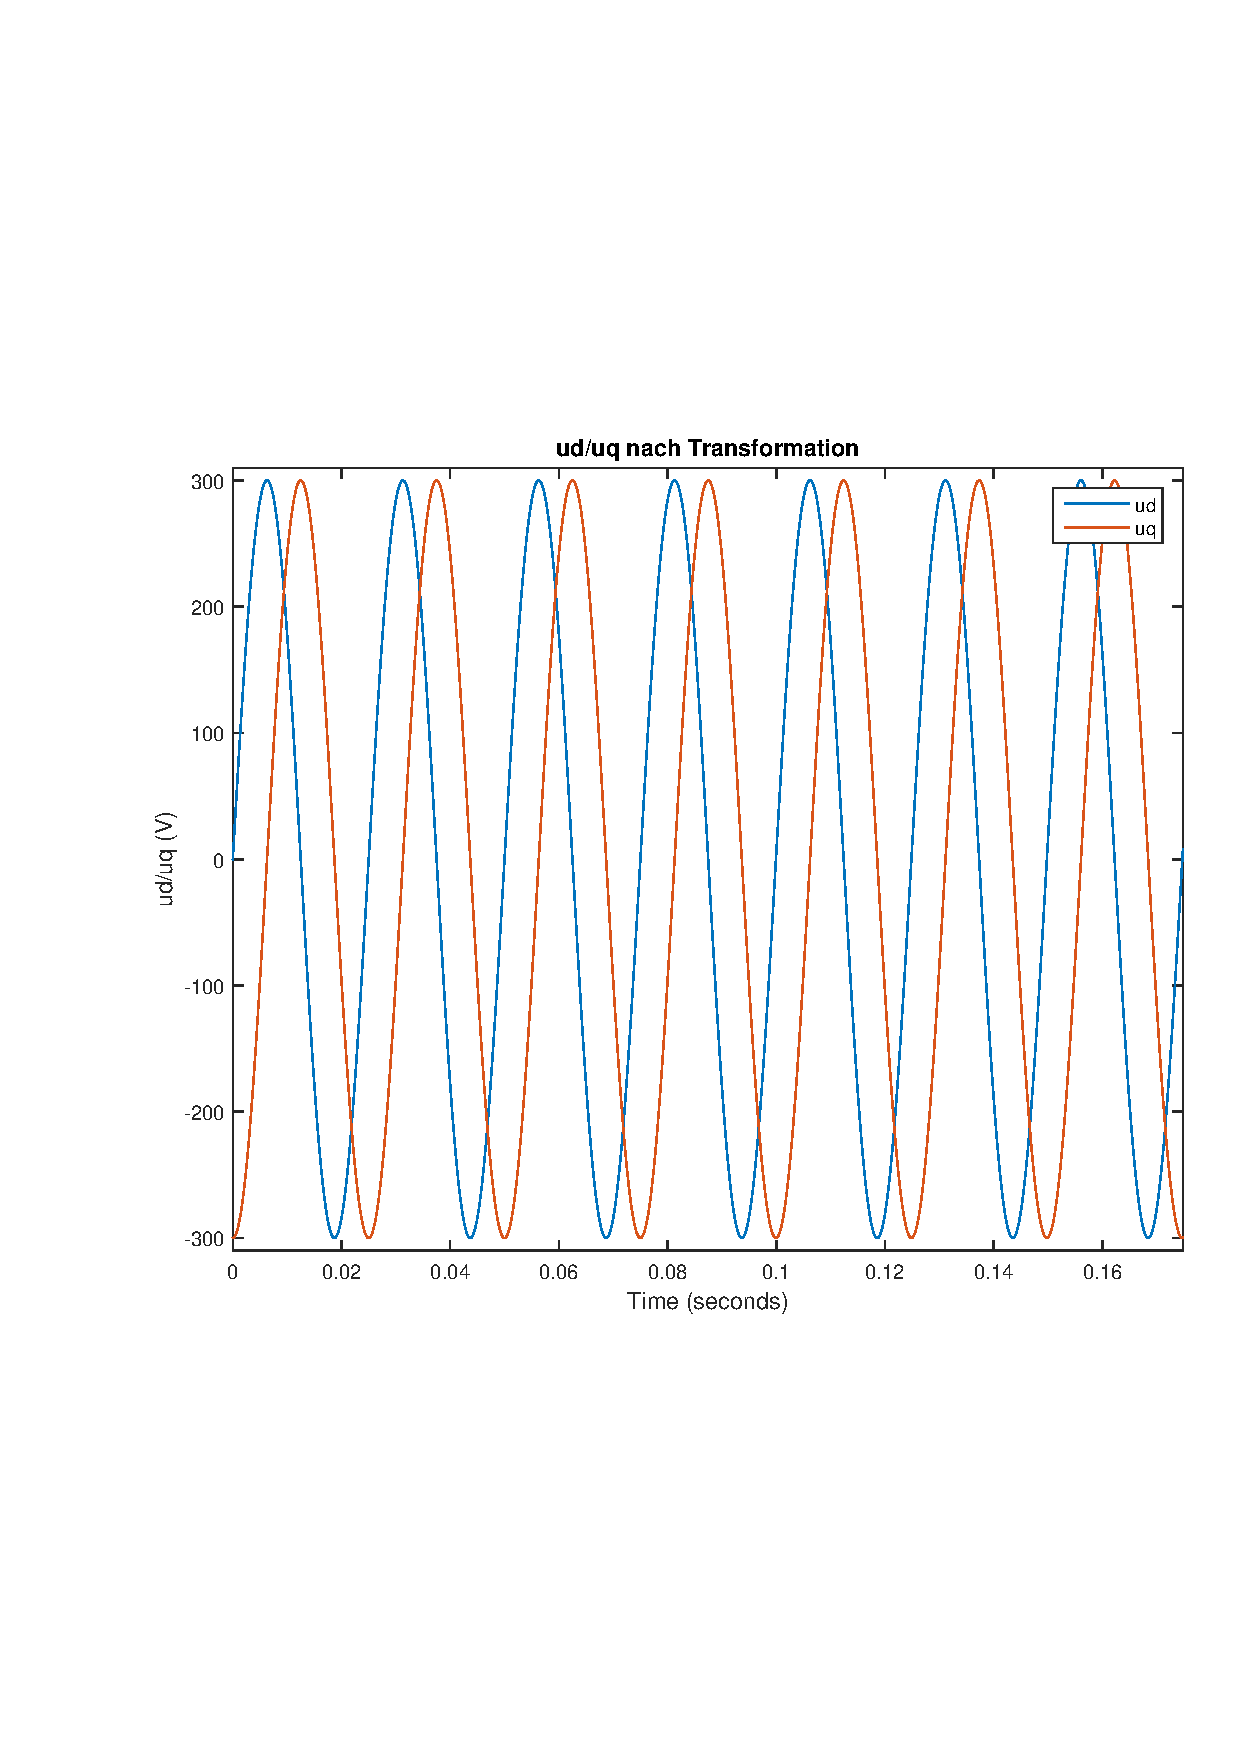
\includegraphics[width=\textwidth]{erg/netz/uduq.pdf}
	\end{minipage}
	\caption{Simulationsergebnisse des starren Netzes. Links: Drehzahl in Abhängig der Zeit (Eingschwingvorgang). Rechts: Clarke-Park-Transformation der Spannungen $(u_\x{d}, u_\x{q})$.}
	\label{fig:n-netz}
\end{figure}

Wie links in Abbildung \ref{fig:n-netz} erkennbar ist, regelt das System die Drehzahl auf \SI{600}{\per\minute}.
Rechts in Abbildung \ref{fig:n-netz} ist der Ausgang der Clarke-Park-Transformation graphisch dargestellt.
Die Transformation soll Gleichgrößen statt Wechselgrößen ausgeben, an dieser Stelle ist das Problem bei der Simulation am starren Netz.
Der zurückgeführte Winkel $\epsilon_\x{RS}$, der PMSM, bewirkt, dass sich die Transformationsausgangsgrößen wie Wechselgrößen verhalten.


\begin{figure}[h!]
	\begin{minipage}[t]{0.5\textwidth}
		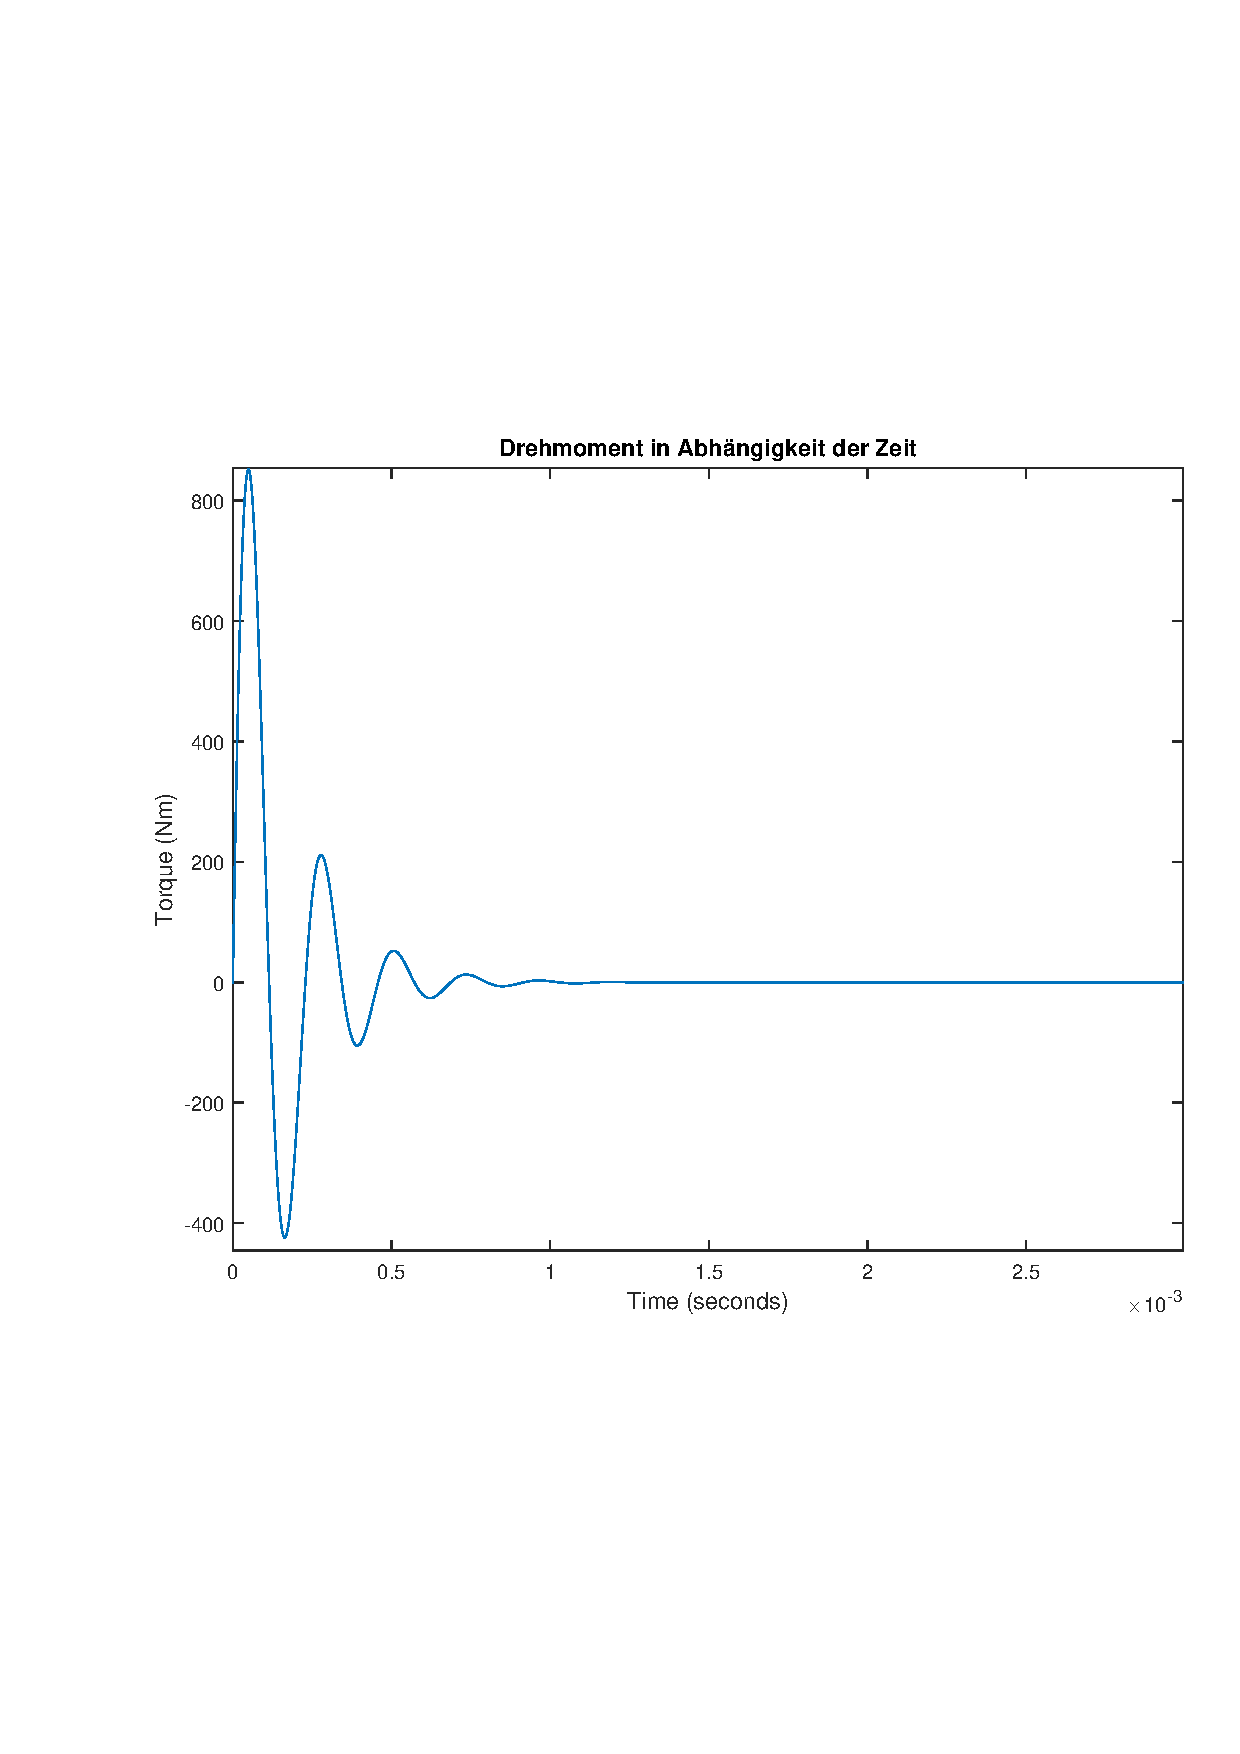
\includegraphics[width=\textwidth]{erg/netz/torque-netz-1.pdf}
	\end{minipage}
	\begin{minipage}[t]{0.5\textwidth} 
		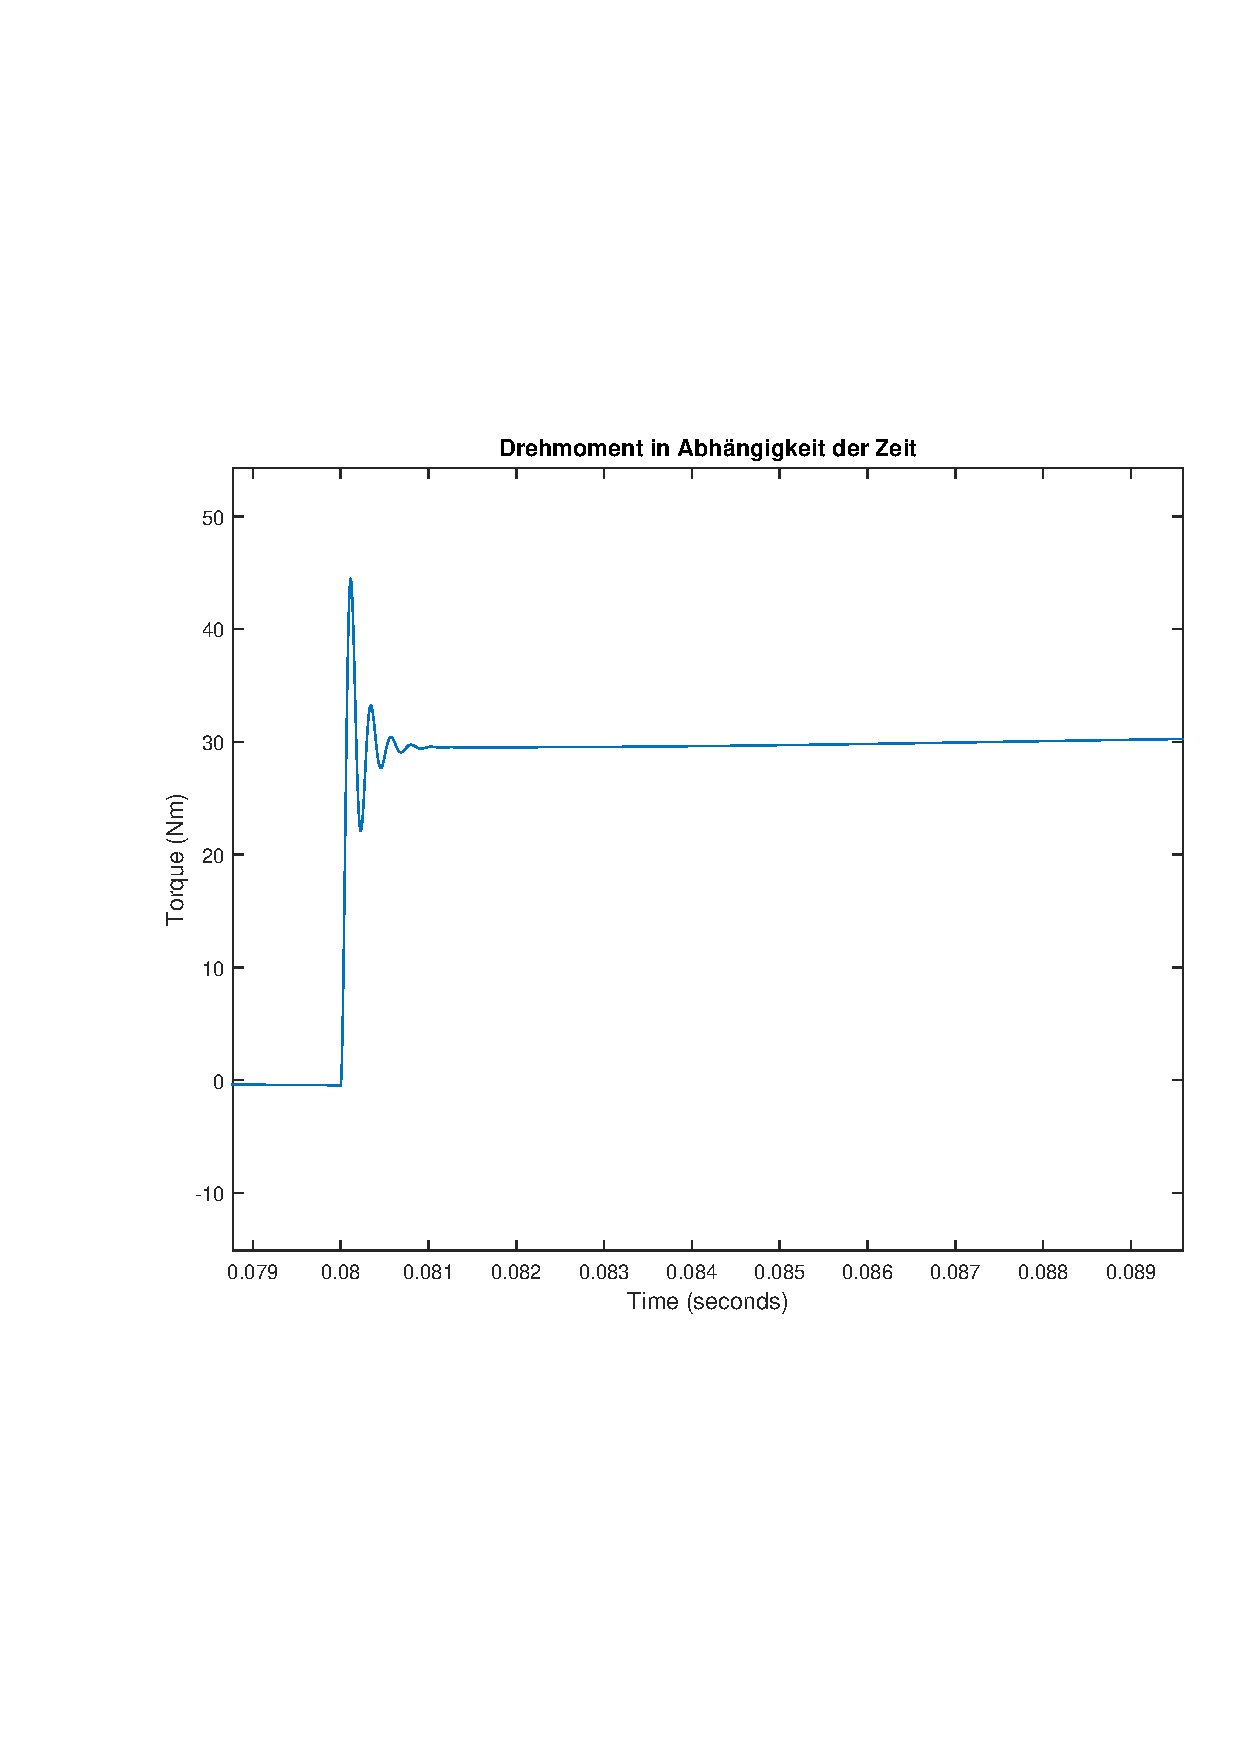
\includegraphics[width=\textwidth]{erg/netz/torque-netz-2.pdf}
	\end{minipage}
	\caption{Ströme der Maschine graphisch dargestellt.}
	\label{fig:mi-netz}
\end{figure}

\newpage

\section{Simulationsergebnisse für die PWM Simulation}\label{sec:sim-pwm}

\begin{figure}[h!]
	\begin{minipage}[t]{0.5\textwidth}
		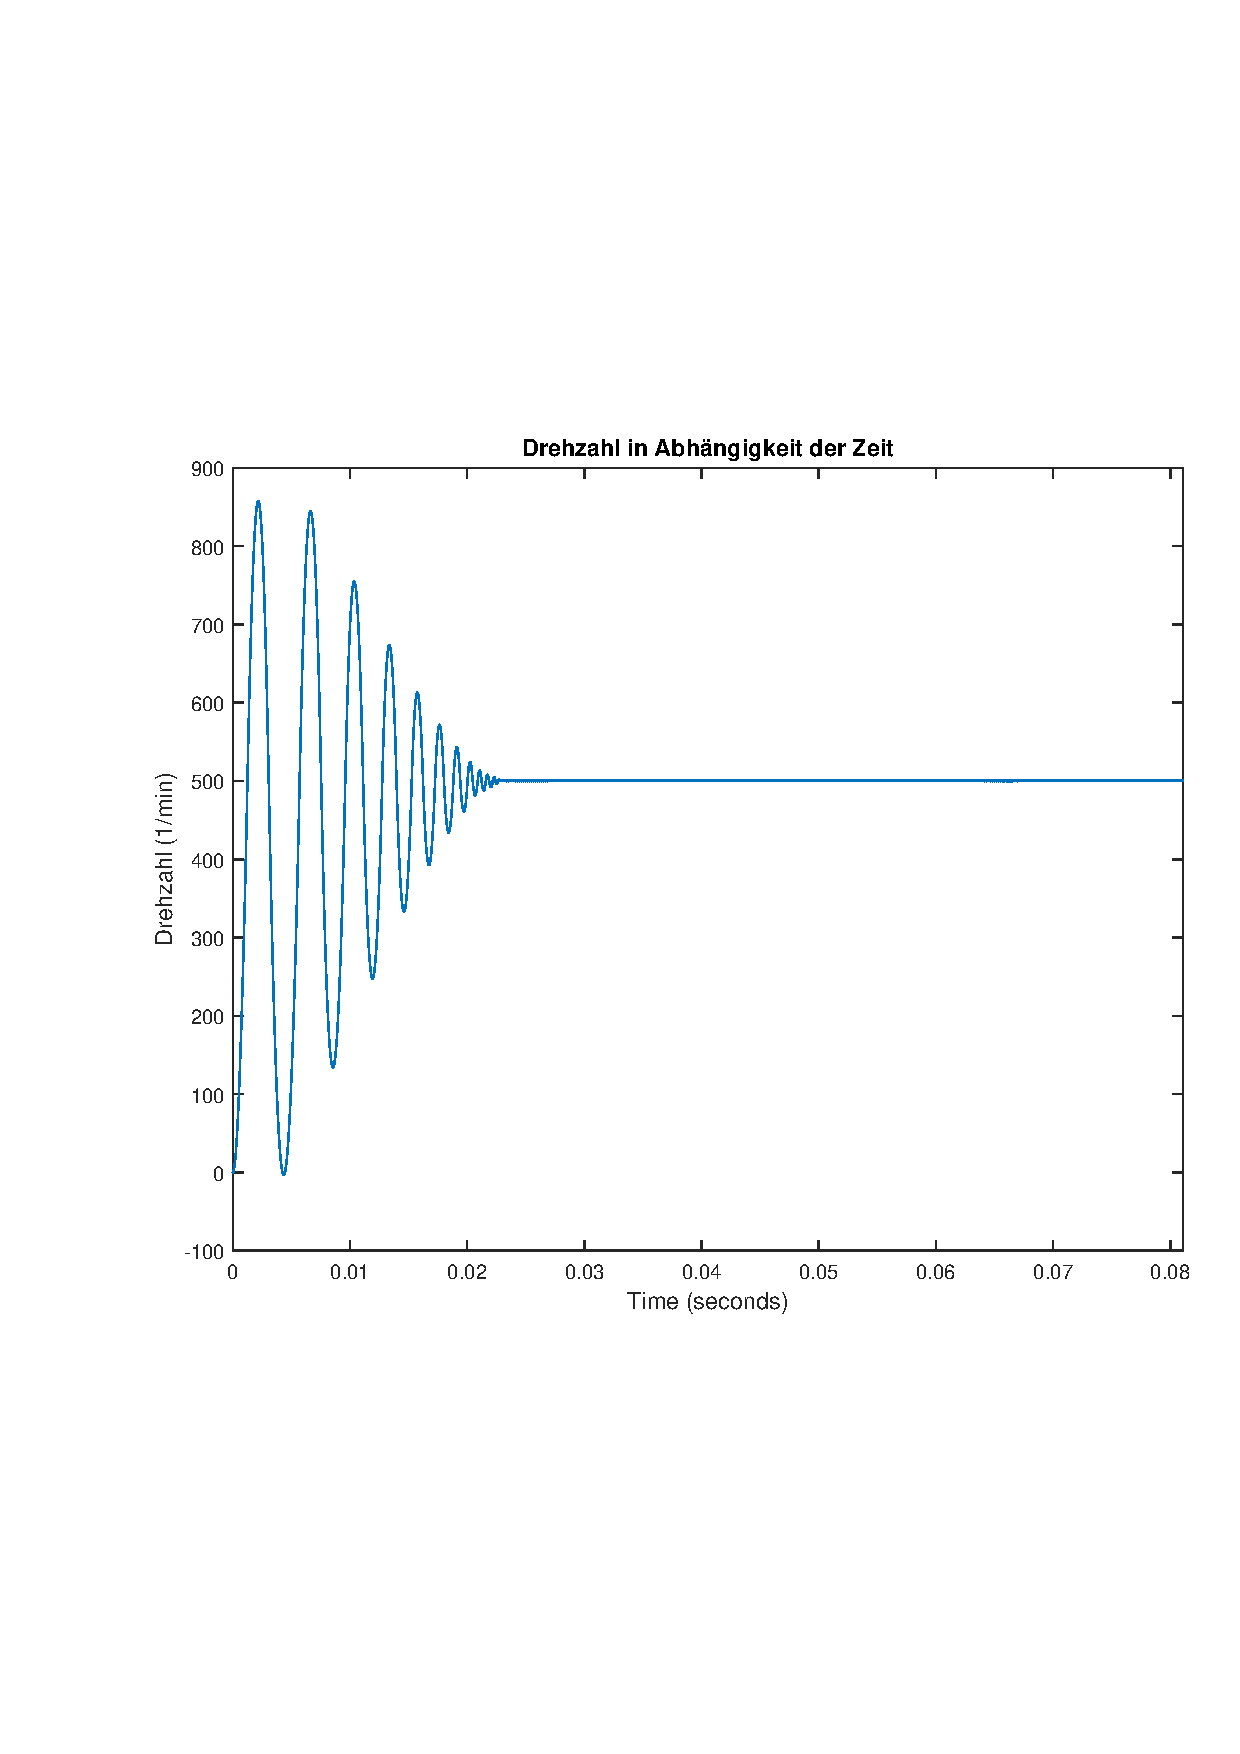
\includegraphics[width=\textwidth]{erg/pwm/rpm-pwm-1.pdf}
	\end{minipage}
	\begin{minipage}[t]{0.5\textwidth} 
		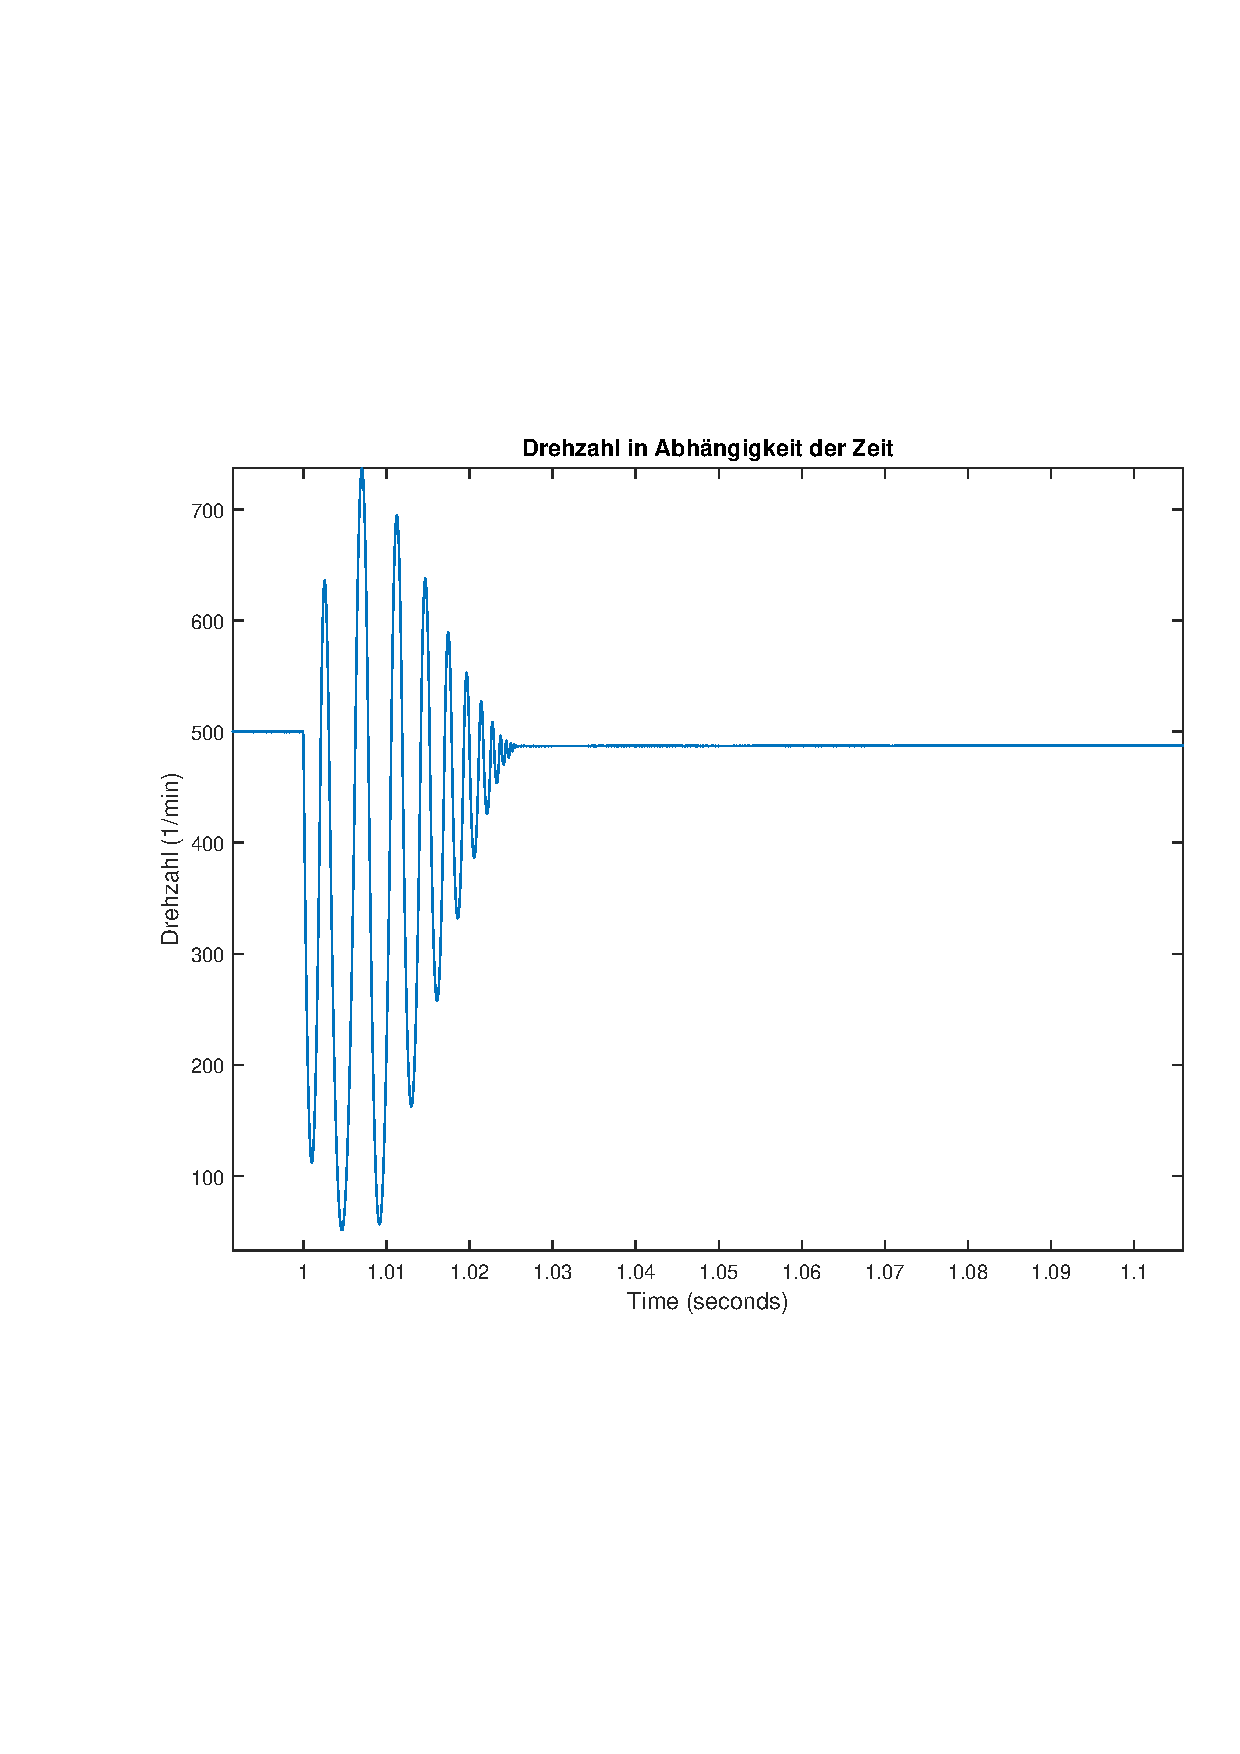
\includegraphics[width=\textwidth]{erg/pwm/rpm-pwm-2.pdf}
	\end{minipage}
	\caption{Drehzahl in Abhängigkeit der Zeit dargestellt. Links: Einschwingvorgang. Rechts: Lastsprung.}
	\label{fig:n-pwm}
\end{figure}

In Abbildung \ref{fig:n-pwm} ist erkennbar, dass die Drehzahl sich auf \SI{500}{\per\minute} einschwingt.

\begin{figure}[h!]
	\begin{minipage}[t]{0.5\textwidth}
		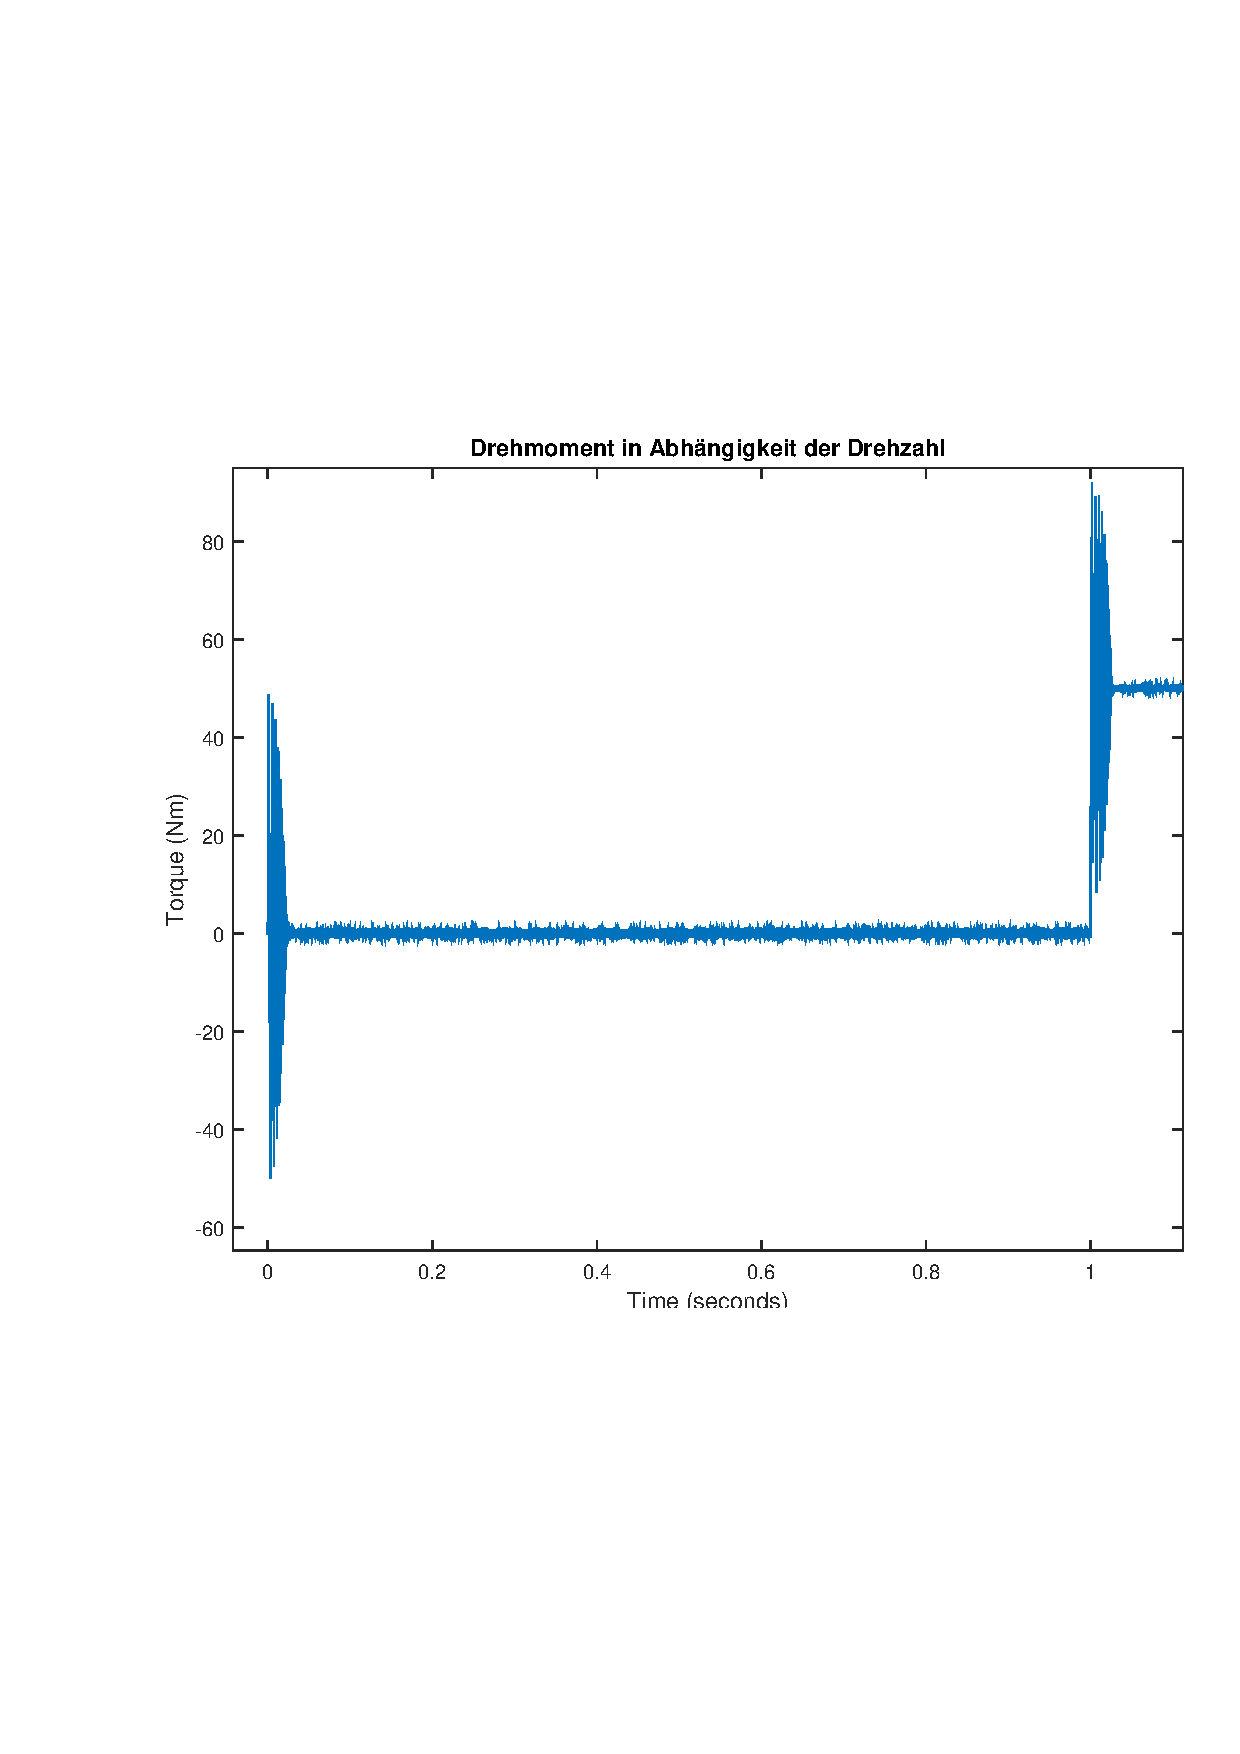
\includegraphics[width=\textwidth]{erg/pwm/torque-pwm-1.pdf}
	\end{minipage}
	\begin{minipage}[t]{0.5\textwidth} 
		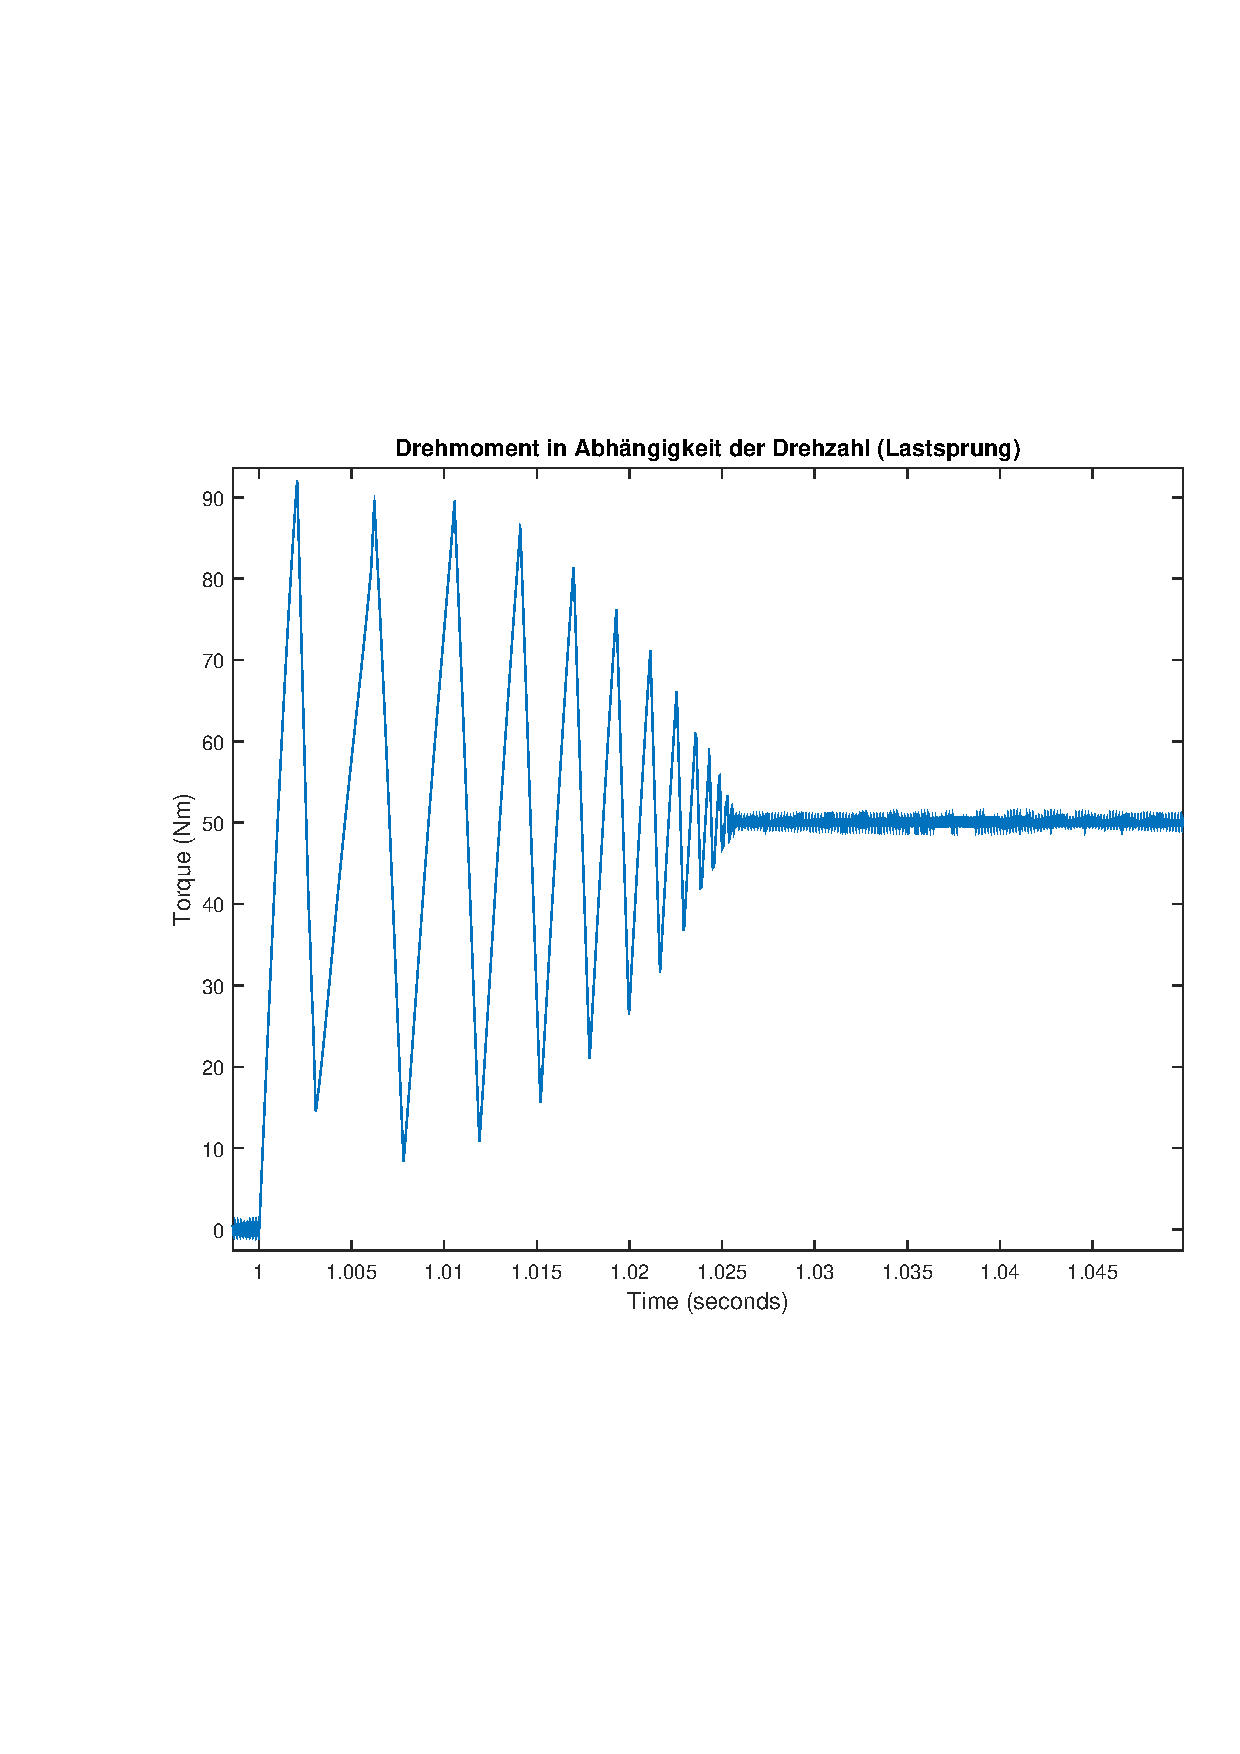
\includegraphics[width=\textwidth]{erg/pwm/torque-pwm-2.pdf}
	\end{minipage}
	\caption{Drehmoment ist in Abhängigkeit der Zeit dargestellt. Links: Einschwingvorgang. Rechts: Lastsprung.}
	\label{fig:mi-pwm}
\end{figure}

Im Gegensatz zur Simulation ohne Netz, entsteht durch die PWM ein sog. \enquote{Torque-ripple} (s.~h.~Abbildung~\ref{fig:mi-pwm}).
Das Drehmoment schwingt sich auf den Sollwert ein, auch nach dem Lastsprung regelt das System diesen so aus, dass sich das Drehmoment relativ schnell auf einem Sollwert von \SI{50}Nm regelt.

\begin{figure}[h!]
	\begin{minipage}[t]{0.5\textwidth}
		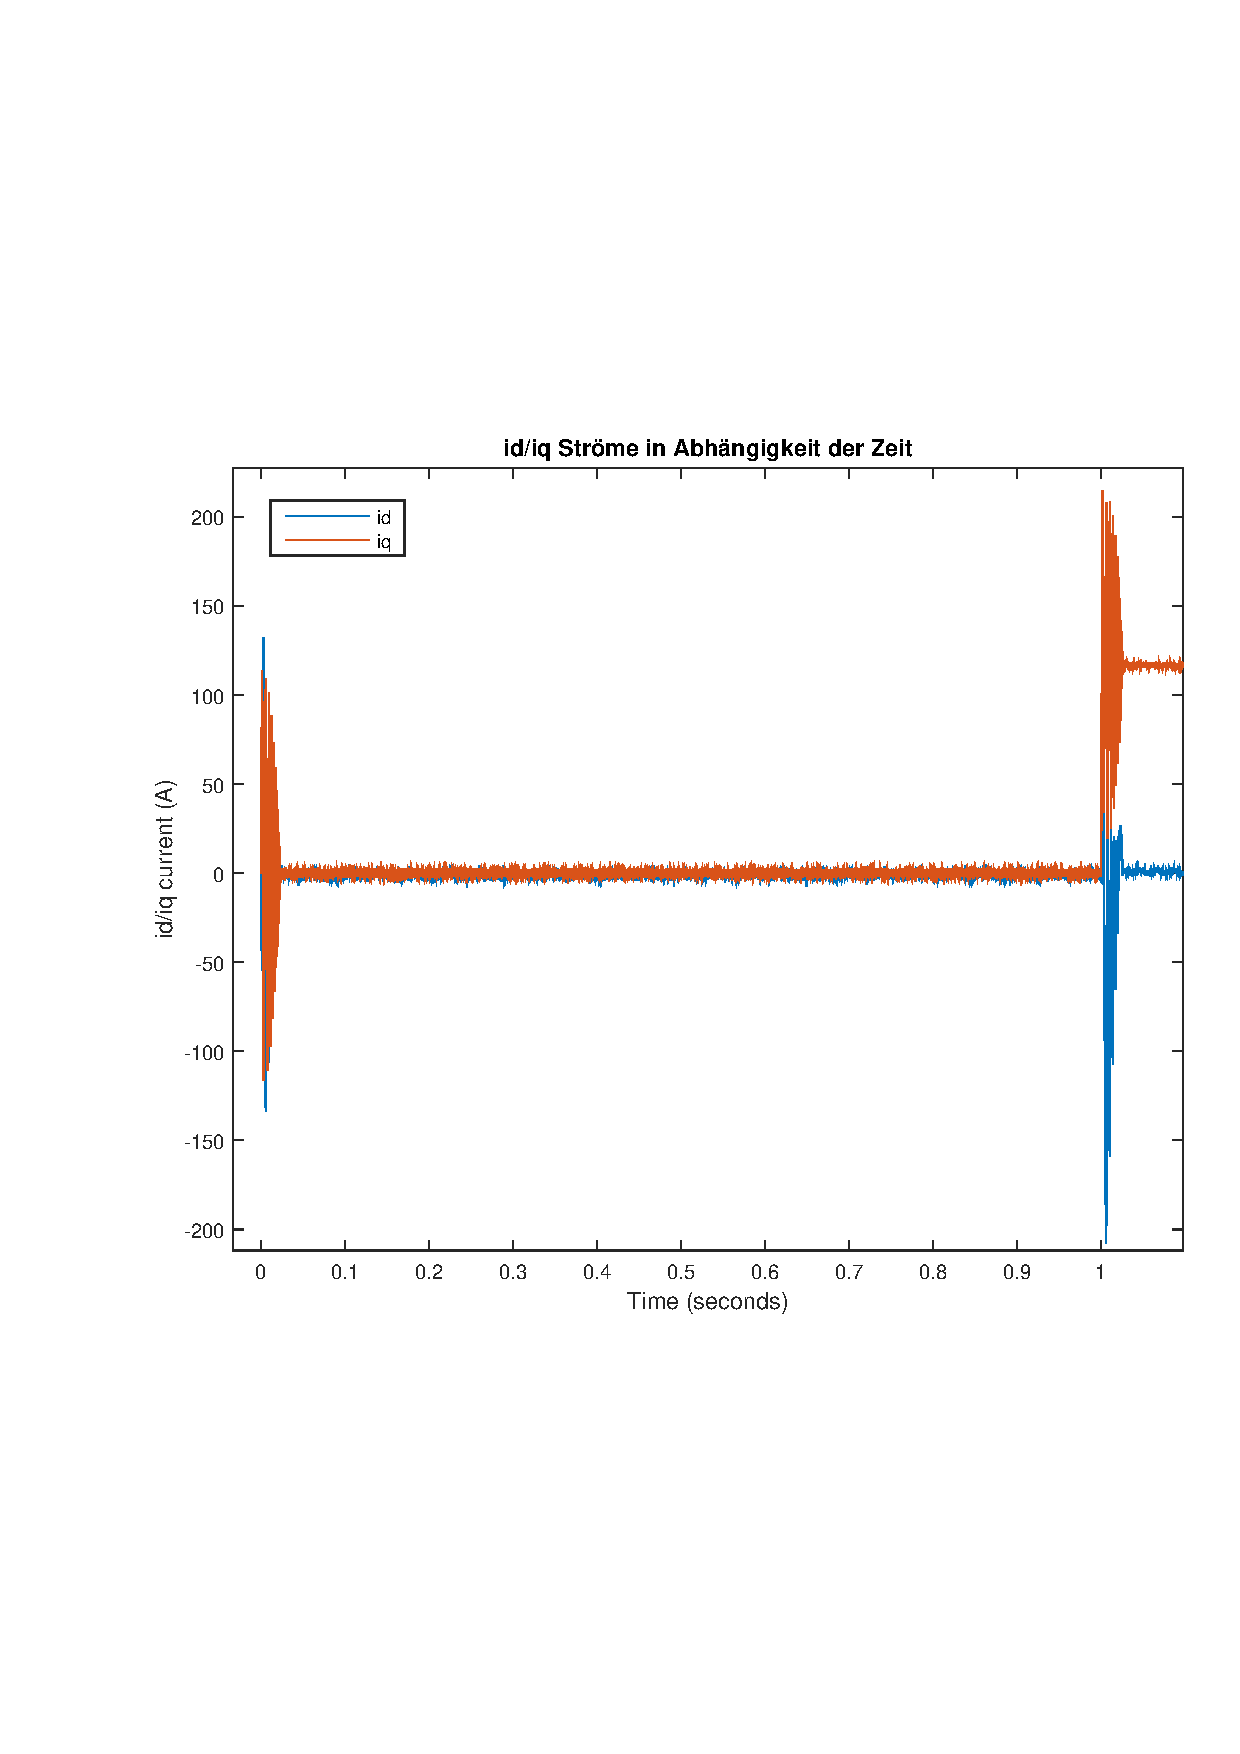
\includegraphics[width=\textwidth]{erg/pwm/current-pwm-1.pdf}
	\end{minipage}
	\begin{minipage}[t]{0.5\textwidth} 
		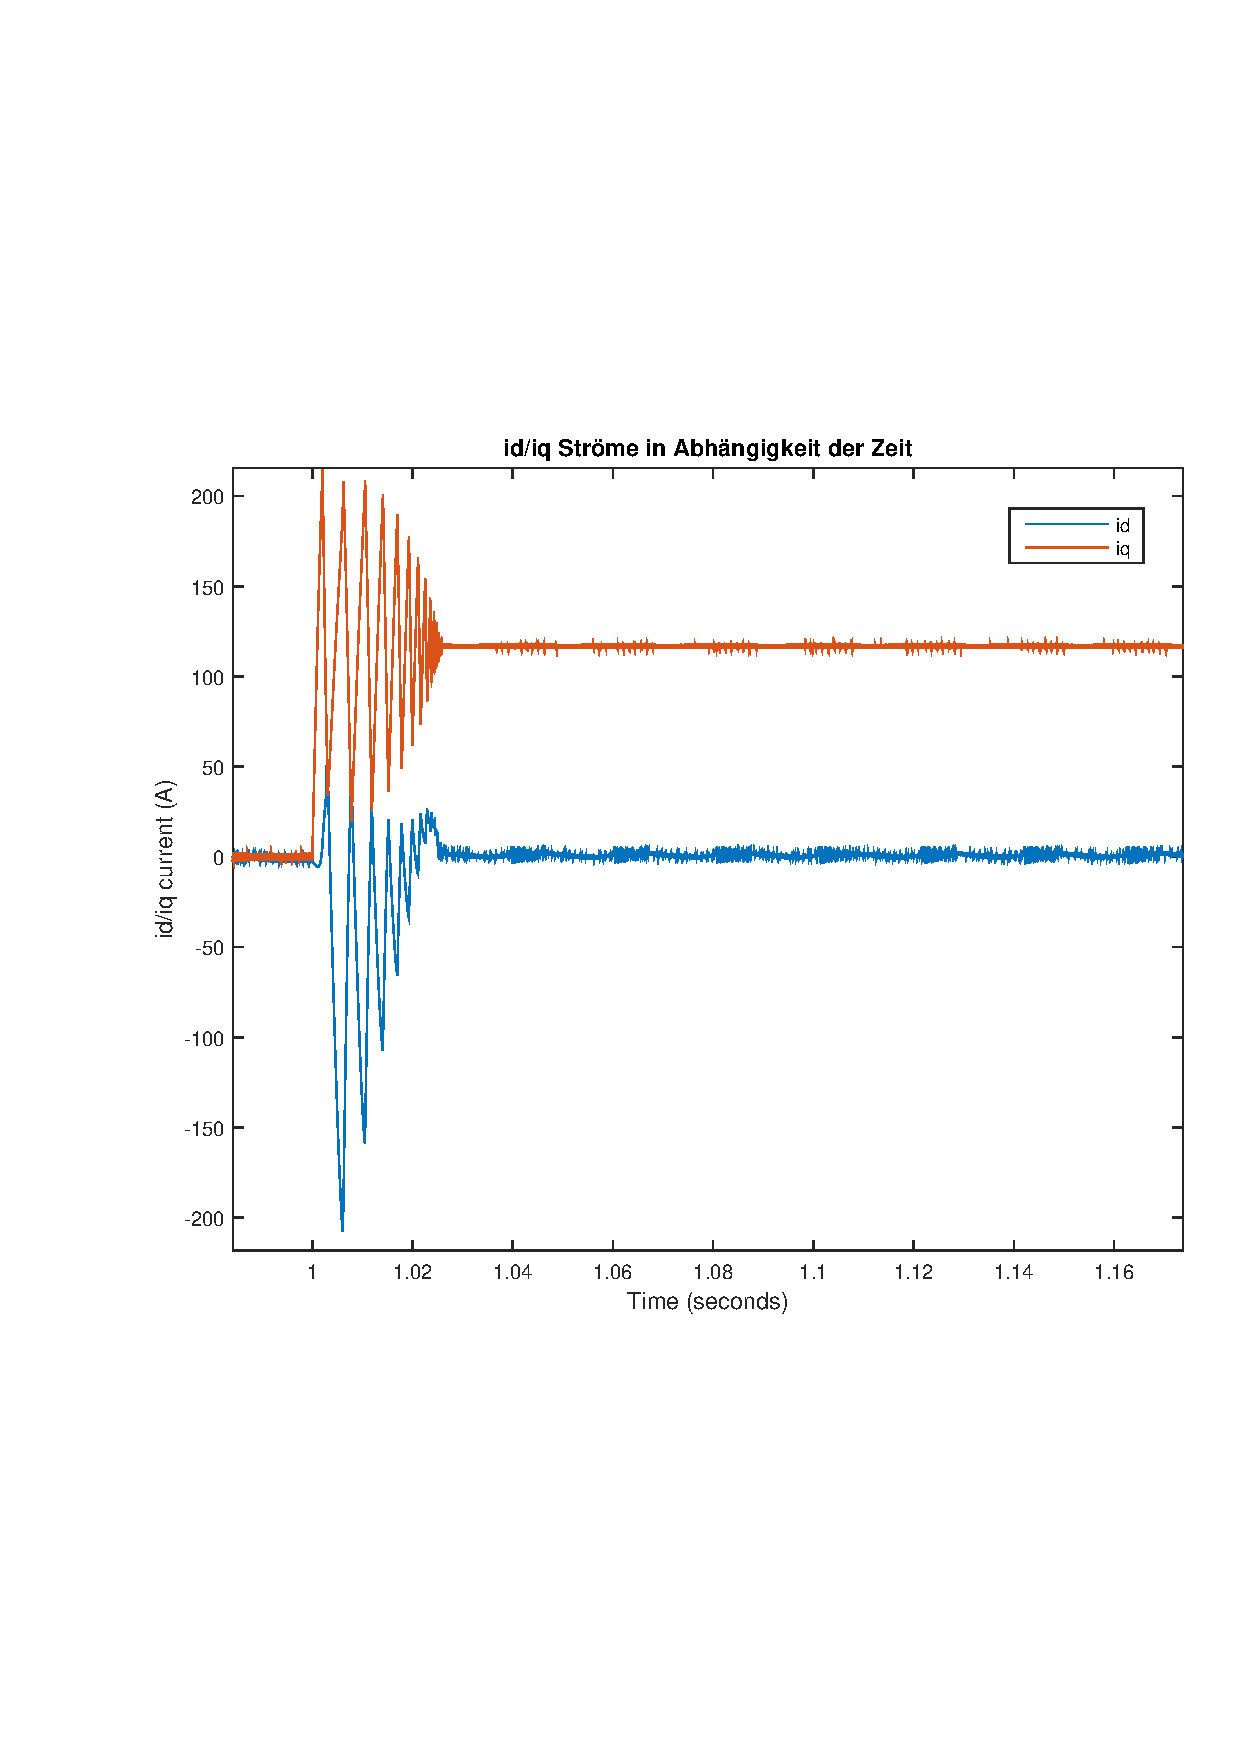
\includegraphics[width=\textwidth]{erg/pwm/current-pwm-2.pdf}
	\end{minipage}
	\caption{Ströme der Maschine graphisch dargestellt.}
	\label{fig:idiq-pwm}
\end{figure}





%%% Local Variables: 
%%% mode: latex
%%% TeX-master: "main"
%%% TeX-open-quote: "\\enquote{"
%%% TeX-close-quote: "}"
%%% LaTeX-csquotes-open-quote: "\\enquote{"
%%% LaTeX-csquotes-close-quote: "}"
%%% End: 
